%Input preamble
%Style
\documentclass[12pt]{article}
\usepackage[top=1in, bottom=1in, left=1in, right=1in]{geometry}
\parindent 22pt
\usepackage{fancyhdr}

%Packages
\usepackage{adjustbox}
\usepackage{amsmath}
\usepackage{amsfonts}
\usepackage{amssymb}
\usepackage{bm}
\usepackage[table]{xcolor}
\usepackage{tabu}
\usepackage{color,soul}
\usepackage{makecell}
\usepackage{longtable}
\usepackage{multirow}
\usepackage[normalem]{ulem}
\usepackage{etoolbox}
\usepackage{graphicx}
\usepackage{tabularx}
\usepackage{ragged2e}
\usepackage{booktabs}
\usepackage{caption}
\usepackage{fixltx2e}
\usepackage[para, flushleft]{threeparttablex}
\usepackage[capposition=top,objectset=centering]{floatrow}
\usepackage{subcaption}
\usepackage{pdfpages}
\usepackage{pdflscape}
\usepackage{natbib}
\usepackage{bibunits}
\definecolor{maroon}{HTML}{990012}
\usepackage[colorlinks=true,linkcolor=maroon,citecolor=maroon,urlcolor=maroon,anchorcolor=maroon]{hyperref}
\usepackage{marvosym}
\usepackage{makeidx}
\usepackage{tikz}
\usetikzlibrary{shapes}
\usepackage{setspace}
\usepackage{enumerate}
\usepackage{rotating}
\usepackage{tocloft}
\usepackage{epstopdf}
\usepackage[titletoc]{appendix}
\usepackage{framed}
\usepackage{comment}
\usepackage{xr}
\usepackage{titlesec}
\usepackage{footnote}
\usepackage{longtable}
\newlength{\tablewidth}
\setlength{\tablewidth}{9.3in}
\setcounter{secnumdepth}{4}

\titleformat{\paragraph}
{\normalfont\normalsize\bfseries}{\theparagraph}{1em}{}
\titlespacing*{\paragraph}
{0pt}{3.25ex plus 1ex minus .2ex}{1.5ex plus .2ex}
\makeatletter
\pretocmd\start@align
{%
  \let\everycr\CT@everycr
  \CT@start
}{}{}
\apptocmd{\endalign}{\CT@end}{}{}
\makeatother
%Watermark
\usepackage[printwatermark]{xwatermark}
\usepackage{lipsum}
\definecolor{lightgray}{RGB}{220,220,220}
%\newwatermark[allpages,color=lightgray,angle=45,scale=3,xpos=0,ypos=0]{Preliminary Draft}

%Further subsection level
\usepackage{titlesec}
\setcounter{secnumdepth}{4}
\titleformat{\paragraph}
{\normalfont\normalsize\bfseries}{\theparagraph}{1em}{}
\titlespacing*{\paragraph}
{0pt}{3.25ex plus 1ex minus .2ex}{1.5ex plus .2ex}

\setcounter{secnumdepth}{5}
\titleformat{\subparagraph}
{\normalfont\normalsize\bfseries}{\thesubparagraph}{1em}{}
\titlespacing*{\subparagraph}
{0pt}{3.25ex plus 1ex minus .2ex}{1.5ex plus .2ex}

%Functions
\DeclareMathOperator{\cov}{Cov}
\DeclareMathOperator{\corr}{Corr}
\DeclareMathOperator{\var}{Var}
\DeclareMathOperator{\plim}{plim}
\DeclareMathOperator*{\argmin}{arg\,min}
\DeclareMathOperator*{\argmax}{arg\,max}

%Math Environments
\newtheorem{theorem}{Theorem}
\newtheorem{claim}{Claim}
\newtheorem{condition}{Condition}
\renewcommand\thecondition{C--\arabic{condition}}
\newtheorem{algorithm}{Algorithm}
\newtheorem{assumption}{Assumption}
\renewcommand\theassumption{A--\arabic{assumption}}
\newtheorem{remark}{Remark}
\renewcommand\theremark{R--\arabic{remark}}
\newtheorem{definition}[theorem]{Definition}
\newtheorem{hypothesis}[theorem]{Hypothesis}
\newtheorem{property}[theorem]{Property}
\newtheorem{example}[theorem]{Example}
\newtheorem{result}[theorem]{Result}
\newenvironment{proof}{\textbf{Proof:}}{$\bullet$}

%Commands
\newcommand\independent{\protect\mathpalette{\protect\independenT}{\perp}}
\def\independenT#1#2{\mathrel{\rlap{$#1#2$}\mkern2mu{#1#2}}}
\newcommand{\overbar}[1]{\mkern 1.5mu\overline{\mkern-1.5mu#1\mkern-1.5mu}\mkern 1.5mu}
\newcommand{\equald}{\ensuremath{\overset{d}{=}}}
\captionsetup[table]{skip=10pt}
%\makeindex

\setlength\parindent{20pt}
\setlength{\parskip}{0pt}

\newcolumntype{L}[1]{>{\raggedright\let\newline\\\arraybackslash\hspace{0pt}}m{#1}}
\newcolumntype{C}[1]{>{\centering\let\newline\\\arraybackslash\hspace{0pt}}m{#1}}
\newcolumntype{R}[1]{>{\raggedleft\let\newline\\\arraybackslash\hspace{0pt}}m{#1}}



%Logo
%\AddToShipoutPictureBG{%
%  \AtPageUpperLeft{\raisebox{-\height}{
\includegraphics[width=1.5cm]{uchicago.png}}}
%}

\newcolumntype{L}[1]{>{\raggedright\let\newline\\\arraybackslash\hspace{0pt}}m{#1}}
\newcolumntype{C}[1]{>{\centering\let\newline\\\arraybackslash\hspace{0pt}}m{#1}}
\newcolumntype{R}[1]{>{\raggedleft\let\newline\\\arraybackslash\hspace{0pt}}m{#1}}

\newcommand{\mr}{\multirow}
\newcommand{\mc}{\multicolumn}

%\newcommand{\comment}[1]{}

%Other parameters
\newcommand{\noutcomes}{95}
\newcommand{\noutcomesexpp}{357}
\newcommand{\noutcomesexpm}{343}
\newcommand{\noutcomesexpf}{355}
\newcommand{\treatsubsabc}{$75\%$}
\newcommand{\treatsubscarec}{$74\%$}
\newcommand{\treatsubscaref}{$63\%$}

%Counts
%Males
\newcommand{\positivem}{$78\%$}
\newcommand{\positivesm}{$29\%$}

%Females
\newcommand{\positivef}{$78\%$}
\newcommand{\positivesf}{$31\%$}

%Counts, control substitution
%Males
\newcommand{\positivecsnm}{$47\%$}
\newcommand{\positivescsnm}{$15\%$}

\newcommand{\positivecsam}{$79\%$}
\newcommand{\positivescsam}{$29\%$}

%Females
%% no alternative
\newcommand{\positivecsnf}{$84\%$}
\newcommand{\positivescsnf}{$55\%$}

%% alternative
\newcommand{\positivecsaf}{$79\%$}
\newcommand{\positivescsaf}{$33\%$}

%Pooled

%Effects
%Males

%Females
\newcommand{\empf}{$8$}
\newcommand{\yearsedf}{$1.7$}



%Pooled

%CBA
%IRR
%Males
\newcommand{\irrm}{$15\%$}
\newcommand{\irrsem}{$5\%$}

%Females
\newcommand{\irrf}{$9\%$}
\newcommand{\irrsef}{$7\%$}

%Pooled
\newcommand{\irrp}{$13\%$}
\newcommand{\irrsep}{$5\%$}

%BC
%Males
\newcommand{\bcm}{$11.24$}
\newcommand{\bcsem}{$4.60$}

%Females
\newcommand{\bcf}{$2.35$}
\newcommand{\bcsef}{$1.09$}

%Pooled
\newcommand{\bcp}{$5.63$}
\newcommand{\bcsep}{$2.15$}

%NPV streams
%Pooled
\newcommand{\parincomenpvp}{$\$119,346$}

%\interfootnotelinepenalty=10000

\newcommand*\leftright[2]{%
  \leavevmode
  \rlap{#1}%
  \hspace{0.5\linewidth}%
  #2}

\newcommand{\orth}{\ensuremath{\perp\!\!\!\perp}}%
\newcommand{\indep}{\orth}%
\newcommand{\notorth}{\ensuremath{\perp\!\!\!\!\!\!\diagup\!\!\!\!\!\!\perp}}%
\newcommand{\notindep}{\notorth}


\externaldocument{abc_comprehensivecba_appendix-pub}
\externaldocument{abc_comprehensivecba_answerstoreferees}

\titlespacing{\section}{0pc}{.35pc}{.35pc}
\titlespacing{\subsection}{0pc}{.35pc}{.35pc}
\titlespacing{\subsubsection}{0pc}{.35pc}{.35pc}

\begin{document}

\begin{titlepage}
\newgeometry{top=.8in, bottom=.8in, left=.8in, right=.8in}


\title{\Large \textbf{Quantifying the Life-cycle \\ Benefits of an Influential Early Childhood Program}\thanks{This research was supported in part by grants from the Robert Wood Johnson Foundation's Policies for Action program, NICHD R37HD065072, the American Bar Foundation, the Buffett Early Childhood Fund, the Pritzker Children's Initiative, NICHD R01HD054702, NIA R01AG042390, and by the National Institute On Aging of the National Institutes of Health under Award Number P30AG024968. The views expressed in this paper are solely those of the authors and do not necessarily represent those of the funders or the official views of the National Institutes of Health. The authors wish to thank Frances Campbell, Craig and Sharon Ramey, Margaret Burchinal, Carrie Bynum, and the staff of the Frank Porter Graham Child Development Institute at the University of North Carolina Chapel Hill for the use of data and source materials from the Carolina Abecedarian Project and the Carolina Approach to Responsive Education. Years of partnership and collaboration have made this work possible. Andr\'{e}s Hojman, Yu Kyung Koh, Sylvi Kuperman, Stefano Mosso, Rodrigo Pinto, Joshua Shea, Jake Torcasso, and Anna Ziff contributed to the analysis in this paper. We thank Bryan Tysinger of the Leonard D. Schaeffer Center for Health Policy and Economics at the University of Southern California for help adapting the Future Adult Model to make the health projections used in this paper. For helpful comments on various versions of the paper, we thank the editor, Harald Uhlig, two anonymous referees, St\'{e}phane Bonhomme, Fl\'{a}vio Cunha, Steven Durlauf, David Figlio, Dana Goldman, Ganesh Karapakula, Magne Mogstad, Sidharth Moktan, Tanya Rajan, Azeem Shaikh, Jeffrey Smith, Chris Taber, Matthew Tauzer, Ed Vytlacil, Jim Walker, Chris Walters, and Matt Wiswall. We benefited from helpful comments received at the Leonard D. Schaeffer Center for Health Policy and Economics in December, 2016, and at the University of Wisconsin, February, 2017. We thank Peg Burchinal, Carrie Bynum, Frances Campbell, and Elizabeth Gunn for information on the implementation of the Carolina Abecedarian Project and the Carolina Approach to Responsive Education and assistance in data acquisition. For information on childcare in North Carolina, we thank Richard Clifford and Sue Russell. The set of codes to replicate the computations in this paper are posted in a repository. Interested parties can request to download all the files. The address of the repository is \url{https://github.com/jorgelgarcia/abccare-cba}. To replicate the results in this paper, contact the first author, who will put you in contact with the appropriate individuals to obtain access to restricted data. The Appendix for this paper is posted on \url{http://cehd.uchicago.edu/ABC_CARE}.}}

\author{
Jorge Luis Garc\'{i}a\\
John E. Walker  Department of Economics\\
Clemson University \\
Social Science Research Institute \\
Duke University \\  \and
James J. Heckman \\
American Bar Foundation \\
Center for the Economics \\
of Human Development \\
The University of Chicago \and
Duncan Ermini Leaf \\
Leonard D. Schaeffer Center \\  for Health Policy and Economics\\
University of Southern California \and
Mar\'{i}a Jos\'{e} Prados \\
Dornsife Center for \\ Economic and Social Research\\
University of Southern California}
\date{First Draft: January 5, 2016\\ This Draft: \today}

\maketitle
\thispagestyle{empty}
\restoregeometry
\end{titlepage}

\singlespacing
\thispagestyle{empty}

\bigskip

\begin{abstract}
\noindent This paper quantifies and aggregates the multiple life-cycle benefits of an influential high-quality early childhood program with outcomes measured through midlife. Guided by economic theory, we supplement experimental data with non-experimental data to forecast the life-cycle benefits and costs of the program. Our point estimate of the internal rate of return is 13.7\% with an associated benefit/cost ratio of 7.3. We account for model estimation and forecasting error and present estimates from extensive sensitivity analyses. This paper is a template for synthesizing experimental and non-experimental data using economic theory to estimate the long-run life-cycle benefits of social programs.
\end{abstract}

\noindent \textbf{Keywords}: Early childhood education, life-cycle benefits, long-term forecasts, program evaluation, rates of return, cost-benefit analysis \\
\noindent \textbf{JEL codes}: J13, I28, C93\\


\bigskip
\begin{tabular}{ll}
Jorge Luis Garc\'{i}a                                          & James J. Heckman \\
John E. Walker                                     & Center for the Economics \\
 Department of Economics                   & of Human Development \\
Clemson University                                       & University of Chicago \\
228 Sirrine Hall                                       & 1126 East 59th Street \\
Clemson, SC 29630                                             & Chicago, IL 60637 \\
Phone: 773-449-0744                                       & Phone: 773-702-0634  \\
Email: jorge.ggmenendez@gmail.com                    & Email: jjh@uchicago.edu \\
                                                                          & \\
Duncan Ermini Leaf                                           & Mar\'{i}a Jos\'{e} Prados \\
Leonard D. Schaeffer Center for                       & Dornsife Center for  \\
Health Policy \& Economics                              & Economic and Social Research \\
University of Southern California                       & University of Southern California \\
635 Downey Way                                              & 635 Downey Way        \\
Los Angeles, CA 90089                                    & Los Angeles, CA 90089 \\
Phone: 213-821-6474                                       & Phone: 213-821-7969 \\
Email: dleaf@healthpolicy.usc.edu                     & Email: prados@usc.edu \\

\end{tabular}

\clearpage

\restoregeometry
\doublespacing
\setcounter{page}{1}
%\pagenumbering{arabic}

\section{Introduction}

\noindent A large body of evidence documents that high-quality early childhood programs boost the skills of disadvantaged children.\footnote{See \citet{Cunha_Heckman_ea_2006_HEE}, \citet{Almond-Currie_2011_JEP}, \citet{Duncan_Magnuson_2013_JEP}, and \citet{Elango_Hojman_etal_2016_Early-Edu} for surveys.} Much of this research reports treatment effects of programs on cognitive test scores, school readiness, and measures of early-life social behavior. A few studies analyze longer-term benefits in terms of completed education, adult health, crime and labor income.\footnote{Examples include: \citet{Heckman_Moon_etal_2010_QE}, \citet{Havnes_Mogstad_2011_AEJEP}, and \citet{Campbell_Conti_etal_2014_EarlyChildhoodInvestments}.} Rigorous evidence on their long-term social efficiency is scarce.\footnote{\citet{Belfield_Nores_etal_2006_JHR} and \citet{Heckman_Moon_etal_2010_RateofReturn} present a life cycle cost-benefit analysis of the Perry Preschool Program. Our approach is more comprehensive in terms of the outcomes analyzed and in providing a general methodology that can be replicated to assess the social efficiency of other programs.}

This paper investigates the social benefits and costs of an influential pair of essentially identical early childhood programs conducted in North Carolina that targeted disadvantaged children. The Carolina Abecedarian Project (ABC) and the Carolina Approach to Responsive Education (CARE)---henceforth ABC/CARE---were evaluated by randomized control trials. Both programs were launched in the 1970s. Participants were followed through their mid 30s. The programs started early in life (at 8 weeks of life) and engaged participants until age 5. They generated numerous positive treatment effects.\footnote{A companion paper, \citet{Garcia_Heckman_Ziff_2018_EER}, reports these treatment effects.} Parents of participants (primarily mothers) received free childcare that facilitated parental employment and adult education. The program has a $13.7\%$ (s.e.\ $3\%$) per-annum tax-adjusted internal rate of return and a $7.3$ (s.e.\ $1.84$) tax-adjusted benefit/cost ratio.

The program is a prototype for many programs planned or in place today.\footnote{Programs inspired by ABC/CARE have been (and are currently being) launched around the world. \citet{Sparling_2010_Highlights} and \citet{Ramey_Ramey_Lanzi_2014_Interventions} list numerous programs based on the ABC/CARE approach. The programs are: Infant Health and Development Program (IHDP) in eight different cities in the U.S. \citep{Spiker-etal_1997_Helping}; Early Head Start and Head Start. \citep{Schneider_McDonald-eds_2007_Scale-Up_Vol-1}; John's Hopkins Cerebral Palsy Study in the U.S. \citep{Sparling_2010_Highlights}; Classroom Literacy Interventions and Outcomes (CLIO) study. \citep{Sparling_2010_Highlights}; Massachusetts Family Child Care Study \citep{Collins_etal_2010_Massachusetts-Study}; Healthy Child Manitoba Evaluation \citep{Healthy_Child_Manitoba_2015_Starting-Early}; Abecedarian Approach within an Innovative Implementation Framework \citep{Jensen_Nielsen_2016_ABC-Programme-Pilot}; and Building a Bridge into Preschool in Remote Northern Territory Communities in Australia \citep{UMonash_Dataset_2015_URL}. Current Educare programs in the U.S. are also based on ABC/CARE \citep{Educare_2014_Research_Agenda,Yazejian_Bryant_2012_Educare}. Appendix~\ref{app:details-educare} lists these Educare programs, all of which implement curricula based on ABC/CARE.} About 19\% of all African-American children would be eligible for ABC/CARE today.\footnote{43\% of African-American children were eligible at its inception.} Implementation of the ABC/CARE program in disadvantaged populations would be an effective, socially efficient policy for promoting social mobility.\footnote{\citet{Garcia_2016_National-Implementation-ECI} estimate that if ABC/CARE were implemented on the current stock of eligible children, the intra-black gap (black disadvantaged relative to black advantaged) in high-school graduation, years of education, employment and labor income at age 30 for females would be reduced by $110\%$, $76\%$, $22\%$, and $30\%$, respectively. It would eradicate the black--white high-school graduation gap, reduce the years of education gap to 0.12 years, reduce the employment gap to 14 percentage points, and reduce the labor income gap to 4,075 USD (2014). For males, the program would eradicate the intra-black high-school graduation gap, reduce the years of education gap to 0.18 years, and reduce the employment gap to 9 percentage points.}

This paper addresses a fundamental problem that arises in evaluating social programs. Few program evaluations have complete life-cycle histories of participants. In our data, the oldest experimental subject is in his/her mid 30s. At issue is determining the life-cycle impact of the program. We forecast the full life-cycle benefits and costs of the program using non-experimental data guided by economic theory.\footnote{\citet{Ridder_Moffitt_2007_hbk_metricsdata} discuss data combination methods. These methods are related to the older ``surrogate marker'' literature in biostatistics (see e.g.,\ \citealp{Prentice_1989_Surrogate_SiM}). However, as noted below, exogeneity is an integral part of the models we estimate, although it is not considered in the statistics literature. That literature does not provide testable predictions for validation of its forecasts as we do.}

As a byproduct, we also address the problem of aggregating evidence from the multiplicity of treatment effects found in ABC/CARE. We estimate economically interpretable aggregates: internal rates of return and benefit/cost ratios that monetize the large array of benefits and costs generated. In constructing these aggregates, we account for model estimation and forecasting error and the welfare cost of taxation to fund programs. Our estimates survive extensive sensitivity analyses.

We construct synthetic cohorts from non-experimental samples. The cohorts are chosen to approximate the life cycles of experimentals in their post-experimental years. We formulate and estimate production functions that predict program treatment effects and assess their within-sample forecast accuracy. Some of the inputs of the estimated production functions are changed by treatment and are measured in both experimental and non-experimental samples. If the production functions mapping inputs to outputs across cohorts are unaffected by treatment (i.e., are ``treatment invariant''), we can safely use them to forecast treatment effects at older ages provided that we accurately forecast the path of future inputs. We test and do not reject treatment invariance in experimental and non-experimental samples that overlap in age.\footnote{See \cite{Hurwicz_1962_structural} for the definition treatment (policy) invariance. We build on the methodology of \citet{Heckman_Pinto_etal_2013_PerryFactor}, who relate intermediate and long-term outcomes in a mediation analysis. However, they do not construct out-of-sample forecasts.} We forecast experimental treatment effects using our estimated production functions applied to non-experimental data with inputs and outputs suitably adjusted for cohort effects.

Our analysis is a template for estimating the life-cycle gains of social experiments for which there is less than full lifetime follow-up. Supplementing experimental data with non-experimental data enhances the information available from social experiments. Using economic theory and econometric methods to generate empirically concordant forecasts enhances the credibility of our estimates.

The quest for long-run estimates from experiments with short-term follow-up has recently led to application of informal procedures for estimating long-term benefits using short-term measures of childhood test scores \citep[e.g.][]{Chetty_Friedman_etal_2011_QJoE,Kline_Walters_2016_QJE}. We show by example that these procedures can give very misleading estimates of true life cycle program benefits.

This paper proceeds in the following way. Section~\ref{section:background} describes the ABC/CARE program. Section~\ref{section:cbamethodology} discusses our methodology for forecasting life-cycle outcomes and the evidence supporting our assumptions. To make matters concrete, we consider in detail how we forecast life cycle labor income. Section~\ref{section:cbapractice} discusses how we forecast other life-cycle outcomes. Section~\ref{section:cbaresults} reports baseline estimates of internal rates of return and benefit/cost ratios and reports an array of sensitivity analyses. Section~\ref{section:bcaestimates} uses our estimates to examine the predictive validity of widely used informal forecasting methods. Section~\ref{section:conclusion} summarizes our findings.

\section{ABC/CARE: Background} \label{section:background}

\noindent The Carolina Abecedarian Project and the Carolina Approach to Responsive Education (ABC/CARE) were enriched childcare programs that targeted the early years of disadvantaged, predominately African-American children in Chapel Hill, Durham, and Raleigh in North Carolina.\footnote{Both ABC and CARE were designed and implemented by researchers at the Frank Porter Graham Center of the University of North Carolina in Chapel Hill.} Appendix~\ref{appendix:background} describes these programs in detail. We summarize their main features here.

The goal of these programs was to enhance the life skills of disadvantaged children. They supported language, motor, and cognitive development as well as socio-emotional competencies considered crucial for school success including task orientation, the ability to communicate, independence, and pro-social behavior.\footnote{\citet{Sparling_1974_Synth_Edu_Infant_SPEECH, Ramey_Collier_etal_1976_CarolinaAbecedarianProject, Ramey_etal_1985_Project-CARE_TiECSE, Wasik_Ramey_etal_1990_CD, Ramey-etal_2012-ABC}.} They also provided free health screenings to treatment-group members with costs of medications borne by the parents.

The design and implementation of ABC and CARE were very similar. Both had two phases, the first of which lasted from birth until age 5. In this phase, children were randomly assigned to treatment. The second phase of the study consisted of home visits from ages 5 through 8 that were assigned by a second-stage randomization. The first phase of CARE, from birth until age 5, had an additional treatment arm of home visits designed to improve home environments.\footnote{\citet{Wasik_Ramey_etal_1990_CD}.}

ABC recruited four cohorts of children born between 1972 and 1976. CARE recruited two cohorts of children, born between 1978 and 1980. For both programs, families of potential participants were referred to researchers by local social service agencies and hospitals at the beginning of the mother's last trimester of pregnancy. Eligibility was determined by a score on a childhood ``risk index'' of disadvantage.\footnote{See  Appendix~\ref{app:eligibility-pop} for details on the construction of the ``risk index'' used to determine eligibility.}

Our analysis uses data from the first phase and pools the ABC treatment group with that of the CARE treatment groups. We do not use the data from the CARE group that only received home visits in the early years. \cite{Campbell_Conti_etal_2014_EarlyChildhoodInvestments} test and do not reject the hypothesis that the CARE data through age 5 (without home visits) and the ABC data through age 5 come from the same distribution.

The initial ABC sample consisted of 120 families. Due to attrition and non-response, the study sample was reduced to 114 subjects: 58 in the treatment group and 56 in the control group. In CARE, the initial sample had 65 families: 23 were randomized to a control group, 25 to a family education treatment group, and 17 to a center-based childcare treatment group that followed ABC protocols.\footnote{There were no randomization compromises in CARE. During preschool, 5 subjects attrited (3 in the treatment group, 1 in the family education group, and 1 in the control group). Details on attrition and non-response are presented in Appendix~\ref{appendix:randomization}.} We use standard weighting methodologies to account for attrition, non-response, and missing data.\footnote{See Appendix~\ref{app:method_partialobs}.}

For both programs, data were collected annually on cognitive and socio-emotional skills, home environments, family structure, and family economic characteristics from birth until age 8. After age 8, data on cognitive and socio-emotional skills, education, and family economic characteristics were collected at ages 12, 15, 21, and 30.\footnote{At age 30, measures of cognitive skills are not available for both ABC and CARE.} In addition, there is information from administrative criminal records, and from a physician-administered medical survey, when the subjects were in their mid 30s.\footnote{See  Appendix~\ref{appendix:data} for a more comprehensive description of the data. There, we document the balance in observed baseline characteristics across the treatment and control groups after dropping the individuals for whom we have no crime or health information. There is substantial missing data for these outcomes, which we address using the methodology exposited in Appendix~\ref{appendix:methodology}.} Many control-group children in both ABC and CARE attended alternative formal childcare arrangements (75\% and 74\% respectively).\footnote{The alternative arrangements were generally lower quality than ABC/CARE (see Appendix~\ref{appendix:tetanus} for details). In our main analysis, we compare treatment- and control-group children, irrespective of take-up of alternatives. In Appendix~\ref{appendix:cbaresultscont}, we address the problem of substitution bias \citep{Heckman_1992_randomization,Heckman_Hohmann_etal_2000_QJE,Kline_Walters_2016_QJE}. We disaggregate our analysis to distinguish treatment effects by type of alternative selected by the control group.}

\section{Forecasting Life-cycle Costs and Benefits: Method} \label{section:cbamethodology}

\noindent To explain our forecasting procedure, the following notation is useful. $W=1$ indicates that parents referred to the program participate in the randomization protocol. $W=0$ indicates otherwise. $R$ indicates randomization into treatment ($R = 1$) or control ($R = 0$). $D$ indicates whether or not a family attends the program. $D= R$ implies compliance with the initial randomization protocol. Lowercase variables $d$ and $r$ denote realizations of $D$ and $R$, respectively. We suppress individual subscripts to avoid notational clutter.

Individuals are eligible to participate in the program if their baseline background variables $\bm{B}\in\mathcal{B}_0$, where $\mathcal{B}_0$ is the set of scores on the childhood risk index that determines program eligibility. Because all of the eligible individuals with the option to participate chose to do so $(W=1\text{, and } D=R)$, we can safely interpret the treatment effects generated by the experiment as average treatment effects for the eligible population and not just average treatment effects for the treated.\footnote{All providers of health care and social services (referral agencies) in the area of the ABC/CARE study were informed of the programs. They referred mothers whom they considered disadvantaged. Eligibility was corroborated before randomization. Conversations with the program staff indicate that all but one of the referred mothers attended and agreed to participate in the initial randomization \citep{Ramey-etal_2012-ABC}.}

Define $\bm{Y}^1_a$ as the outcome vector at age $a$ for the treated. $\bm{Y}^0_a$ is the age-$a$ outcome vector for the controls. At age $a$ the vector of average treatment effects for the population for which $\bm{B}\in\mathcal{B}_0$ is:

\begin{equation}
\bm{\Delta}_a  := \mathbb{E} \left[ \bm{Y}^1_a - \bm{Y}^0_a | W = 1 \right] = \mathbb{E} \left[\bm{Y}^1_a - \bm{Y}^0_{a} | \bm{B} \in \mathcal{B}_0 \right]. \label{eq:mainte}
\end{equation}\
%
Randomization identifies this parameter in the experimental sample.

\subsection{Using Economic Models to Make Forecasts}

\noindent This paper uses economic models to generate unbiased, out-of-sample forecasts of $\bm{\Delta}_a$. We use a structural production function (mediation) model for treatment ($D=1$) and control ($D=0$) outcomes at age $a$ in sample $k \in \{e,n\}$, where $e$ denotes membership in the experimental sample and $n$ denotes membership in a non-experimental (auxiliary) sample. The vector of production functions for output $\bm{Y}^d_{k,a}$ is:
\begin{equation}
\bm{Y}^d_{k,a} = \bm{\phi}^d_{k,a} (\bm{X}^d_{k,a}, \bm{B}_k) \ + \ \bm{\varepsilon}^d_{k,a},  \label{eq:outcome} \\
\end{equation}
$d \in\{0,1\},  k\in\{e,n\}, a\in\{1,\dots,\bar{A}\}$ where $\bm{\phi}^d_{k,a}\left( \cdot, \cdot \right)$ is a vector of structural production relationships mapping inputs $\bm{X}^d_{k,a}, \bm{B}_k$ into outputs holding the error term $\bm{\varepsilon}^d_{k,a}$ fixed.\footnote{Fixing and conditioning are fundamentally different concepts. See \cite{Haavelmo_1943_Econometrica} and \citet{Heckman_Pinto_2015_EconometReviews} for discussions.} $ \bm{B}_k$ are baseline variables not affected by treatment. $\bm{X}^d_{k,a}$ are variables potentially affected by treatment. $\bar{A}$ is the oldest age considered in our analysis. In the experiment we analyze, participants are observed through age $a^*< \bar{A}$.

The relationship between the inputs $\bm{X}^d_{k,a}, \bm{B}_k$ and outputs $\bm{Y}^d_{k,a}$ can, in principle, differ between experimental and non-experimental samples although in our data this is not the case. Equation~\eqref{eq:outcome} characterizes the outcomes of the two treatment regimes in any sample, including a non-experimental sample with no direct empirical counterpart for the case $d = 1$. We present conditions for identifying and estimating $\bm{\phi}^d_{k,a}\left( \cdot, \cdot \right)$ in non-experimental samples. A crucial condition is that for fixed values of inputs $\bm{X}^d_{k,a} = \bm{x}, \bm{B}_k = \bm{b}$ there are no differences in the technologies and in the distributions of $\bm{\varepsilon}_{k,a}^d$ across treatment regimes and samples. We first formalize this assumption and then remark on its content.

\onehalfspacing

\begin{assumption} \label{ass:summary} \textbf{Structural Invariance}
For all $\bm{x}, \bm{b} \in supp(\bm{X}^d_{k,a}, \bm{B}_k), k \in \{e,n\}$, and $a \in \{1,\dots,\bar{A}\}$
\begin{subequations}
\begin{align}
\bm{\phi}_{k,a}^0 \left( \bm{x}, \bm{b} \right) &= \bm{\phi}_{k,a}^1 (\bm{x}, \bm{b}) \nonumber \\                                                                      &= \bm{\phi}_{a} (\bm{x}, \bm{b}), \label{eq:crucialres}
\end{align}
%
where $\bm{\phi}_{a}(\bm{x}, \bm{b})$ is the common structural function (across $d$ and $k$) generating the deterministic portion of the effect of $ \bm{B}_k=\bm{b}, \bm{X}^d_{k,a}=\bm{x}$ on outcomes and
%
\begin{eqnarray}
F_{k,a}^0 \left( \cdot | \text{\textbf{ Fix }} \bm{X}_{k,a}^d = \bm{x}, \bm{B}_{k} = \bm{b} \right) &=& F_{k,a}^1 \left( \cdot  | \text{\textbf{ Fix }} \bm{X}_{k,a}^d = \bm{x}, \bm{B}_{k} = \bm{b} \right) \nonumber \\
  &=&  F_{a} \left( \cdot  | \text{\textbf{ Fix }} \bm{X}_{k,a}^d = \bm{x}, \bm{B}_{k} = \bm{b}  \right), \label{eq:strucinvarianceF}
\end{eqnarray}
\end{subequations}
where $F_{k,a}^j \left( \bm{z} | \text{\textbf{ Fix }} \bm{\Omega} = \bm{\omega} \right)$ denotes the distribution of $\bm{Z}$ for $\bm{\Omega}$ fixed at $\bm{\omega}$ and $F_a \left( \bm{z} | \text{\textbf{ Fix }} \bm{\Omega} = \bm{\omega} \right)$ is the distribution of the errors of the production functions that are assumed to be common across treatment regimes and samples, given $\text{\textbf{ Fix }} \left( \bm{X}_{k,a}^d = \bm{x}, \bm{B}_{k} = \bm{b} \right)$. $\square$
\end{assumption}

We clarify Assumption~\ref{ass:summary} with three remarks.

\begin{remark} \textbf{There are Two Distinct Aspects of Structural Invariance}
Assumption~\ref{ass:summary} has two distinct aspects that can be resolved further into two separate assumptions: (i) structural relationships and distributions evaluated at the same arguments have identical values for treatment and control groups in the experimental sample, and (ii) analogous conditions hold across the experimental and non-experimental samples. Condition (ii) enables analysts to simulate treatment and control outcomes in non-experimental samples.
\end{remark}

\begin{remark} \label{remark:cohort} \textbf{Accounting for Cohort Effects}
A second aspect of Assumption~\ref{ass:summary}, that the structural relationships and distributions are identical in the experimental and non-experimental samples, embeds an implicit assumption about the absence of cohort effects. In particular, a structural function $\bm{\phi}_{n,a}^d \left( \bm{x}, \bm{b} \right)$ or distribution $F^d_{n,a} \left(\bm{z} | \text{ \text{\textbf{Fix}} } \bm{\Omega} = \bm{\omega}\right)$, which we identify and estimate in the non-experimental sample with subjects who are older than those in the experimental sample, is a valid tool for forecasting the experimental sample at older ages currently out of the age range of the experiment. Note that this does not mean that there are no cohort effects in the outcome of interest, $\bm{Y}^d_{k,a}$. Instead, it means that there are no cohort effects in the \textbf{mapping} between $\bm{X}_{k,a}, \bm{B}_k$ and $\bm{Y}_{k,a}^d$, $k \in \{e,n\}$.
\end{remark}

\doublespacing
To test Assumption~\ref{ass:summary} in the experimental and non-experimental samples and to make accurate forecasts at age $a > a^*$, we require the common support conditions that we now formalize. They are tested in Appendix~\ref{app:containsupport}.

\onehalfspacing
\begin{assumption} \label{ass:contain} \textbf{Support and Input Forecast Conditions}
For $a \in \{ 1, \ldots, \bar{A} \}$ and $d \in \{0,1\}$
\begin{equation}
supp( \bm{Y}_{e,a}^d, \bm{X}^d_{e,a}, \bm{B}_e, \bm{\varepsilon}_{e,a} ) \subseteq supp( \bm{Y}_{n,a}^d, \bm{X}^d_{n,a}, \bm{B}_n, \bm{\varepsilon}_{n,a} ).
\end{equation}
We further require that the path of inputs in the post-treatment lives of the experimental treatments and controls have counterparts in the non-experimental sample. This includes accounting for cohort effects.
\end{assumption}

\doublespacing
To make the discussion specific, we now consider how one can use this framework to forecast life-cycle labor income.

\subsection{Forecasting Labor Income} \label{sec:forecasting}

\noindent \textbf{Step 1.\ Constructing a Synthetic Cohort.} We use the Children of the National Longitudinal Survey of Youth (CNLSY) to construct a synthetic cohort from ages 21 to 29. We use both the National Longitudinal Survey of Youth 1979 (NLSY79) and the Panel Study of Income Dynamics (PSID) to construct a synthetic cohort from ages 29 to 67. Whenever we use the NLSY79 and PSID together, we combine samples. Thus we use three non-experimental datasets to obtain information across the life cycle. We satisfy support conditions.\footnote{See Appendix~\ref{app:containsupport}.}

Because we do not observe each element of the eligibility index discussed in Section~\ref{section:background}, we approximate $\bm{B}_{n} \in \mathcal{B}_0$. We delimit the sample to include observations satisfying the following criteria: (i) \textbf{NLSY79:} Black, labor income less than \$300,000 (2014 USD) in any given year, birth year between 1957 and 1965; (ii) \textbf{PSID:} Black, labor income less than \$300,000 (2014 USD), birth year between 1945 and 1981; and (iii) \textbf{CNLSY:} Black, labor income less than \$300,000 (2014 USD) in any given year, birth year between 1978 and 1983.

We weight each individual in the non-experimental samples according to his/her resemblance to the individuals in the experimental sample.\footnote{We use Mahalanobis' matching Algorithm~\ref{alg:match} (see Appendix~\ref{appendix:methodology}).} Baseline pre-treatment match variables are: year of birth, gender, and number of siblings at baseline. All are available in the non-experimental datasets. This procedure generates a synthetic cohort in the non-experimental sample for subsequent analysis in our structural forecasting procedure.

By design, there is no treatment effect in the non-experimental sample. Matching to the experimental sample is executed using baseline variables not affected by treatment in the experimental sample. Figure~\ref{figure:controltests} demonstrates that the synthetic cohort is comparable to the non-experimental sample for which $\bm{B}_{n} \in \mathcal{B}_0$. At age 30, average observed labor income for the control group in the experimental sample coincides with average labor income for the synthetic cohort.\footnote{We observe labor income in the experimental samples at ages 21 and 30. We use the data at age 21 to initialize our forecasting model and hence cannot use it for testing our forecast.}

\begin{sidewaysfigure}[!htbp]
\centering
\caption{Labor Income Profile, Disadvantaged Individuals and Synthetic Cohort Constructed by Matching in the Auxiliary Samples}\label{figure:controltests}
\begin{subfigure}[h]{0.5\textwidth}
		\centering
		\caption{Males}
		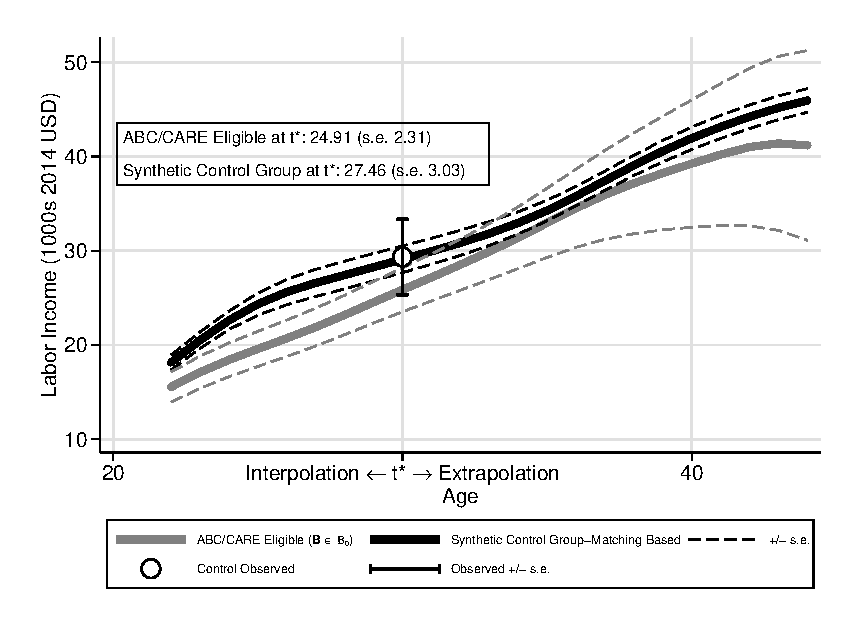
\includegraphics[width=\textwidth]{output/abccare_disad_1.eps}
\end{subfigure}%
\begin{subfigure}[h]{0.5\textwidth}
		\centering
		\caption{Females}
		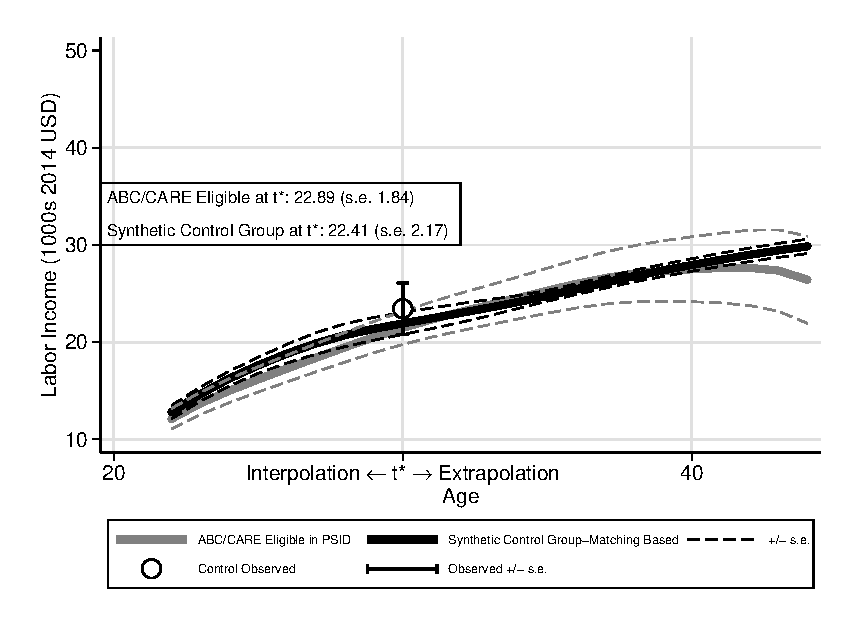
\includegraphics[width=\textwidth]{output/abccare_disad_0.eps}
\end{subfigure}
\footnotesize \justify
Note: Panel (a) displays the forecast labor income for males in the auxiliary samples for whom $\bm{B} \in \mathcal{B}_0$, i.e., ABC/CARE eligible, and for the synthetic cohort we construct based on the method proposed in this section. We combine data from the Panel Study of Income Dynamics (PSID), the National Longitudinal Survey of Youth 1979 (NLSY79), and the Children of the National Longitudinal Survey of Youth 1979 (CNLSY79). We highlight the observed labor income at oldest $a^*$ (age 30) for the ABC/CARE control-group participants. We stop at age 45 for want of data to compute the childhood risk index defining $\bm{B} \in \mathcal{B}_0$ in the auxiliary samples. Panel (b) displays the analogous figure for females. Standard errors are based on the empirical bootstrap distribution. $a^*$ is the oldest age in the experimental sample.
\end{sidewaysfigure}

\textbf{Step 2. Establishing Exogeneity of Inputs.} Forecasting does not require that we take a position on the exogeneity of $\bm{X}^d_{k,a}$ for $k \in \{e,n\}$ and $a \in \{ a, \ldots \bar{A} \}$ with respect to labor income. Estimated structural models with biased parameters can still give reliable forecasts if relationships between observed and unobserved variables are the same within sample and in the forecast sample.\footnote{See \cite{Liu-etal-2016-USC-Data-Models}.  Conditions~\ref{cond:cond1} to~\ref{cond:cond3} in Appendix~\ref{appendix:incomplete} spell out the requirements.} However, exogeneity facilitates the use of economic theory to interpret treatment effects, to forecast outcomes in samples where inputs are manipulated differently than in the experimental sample, and to test the validity of the construction of our synthetic cohort. Exogeneity also makes identification of $\bm{\phi}^d_{k,a}\left( \cdot, \cdot \right)$ in the non-experimental sample straightforward. Assumption~\ref{ass:exog} formalizes a strong form of the exogeneity condition.

\onehalfspacing
\begin{assumption}\label{ass:exog} \textbf{Exogeneity}
Let $\{ 1, \ldots, \bar{A} \}$ index the periods of a life cycle. For all $a, a'' \in \{ 1, \ldots, \bar{A} \}$ and for $d, d' \in \{0,1\}$,
\begin{equation}
\bm{\varepsilon}^d_{k,a} \indep \bm{X}^{d^{\prime}}_{k,a^{''}} | \bm{B}_k = \bm{b}
\end{equation}
for all $\bm{b}$ in the support of $\bm{B}_k, \: k \in \{e,n\}$, where ``$\bm{M} \indep \bm{N}|\bm{Q}$'' denotes independence of $\bm{M}$ and $\bm{N}$ given $\bm{Q}$. $\square$
\end{assumption}
\doublespacing
Below we discuss how this condition can be weakened and unbiased forecasts can still be obtained.

To appreciate the benefit of Assumption~\ref{ass:exog}, consider the following example. Suppose that years of education is a component of $\bm{X}^{d'}_{k,{a''}}$. The joint distribution of $\bm{\varepsilon}_{k,a}^d$ and $\bm{X}^{d'}_{k,{a''}}$ can differ substantially across experimental and non-experimental samples. In the experimental sample, years of education are boosted by treatment, which is randomly assigned. In the non-experimental samples, however, there is no experimental variation. Individuals with high observed levels of education could have high values of $\bm{\varepsilon}_{k,a}^d$ due to omitted ability. This creates a fundamentally different dependence between $\bm{\varepsilon}_{k,a}^d$ and $\bm{X}_{k,{a''}}^{d'}$ in the non-experimental sample. Assumption~\ref{ass:exog} avoids this problem when making forecasts. Below, we establish that our forecasts based on this assumption are concordant with forecasts from approaches that do not necessarily require Assumption~\ref{ass:exog}.

\textbf{Step 3. Determining Inputs.} Analysis of the non-experimental data reveals that the inputs determining labor income under Assumption~\ref{ass:exog} are: average PIAT achievement score from ages 5 to 7, completed education, labor income at age 21, and lagged labor income. Appendix Table~\ref{table:predlaborincome} shows that these variables predict labor income. Appendix~\ref{app:containsupport} shows that there is common support across datasets. We report tests for endogeneity of these variables in the experimental and auxiliary samples used in this paper in Appendix~\ref{appendix:methodology}.\footnote{These tests assume that $\bm{\varepsilon}_{k,a}^d, k \in \{e,n\}$, follows a factor structure. Factor structure models are widely used in structural estimation of production functions of skills during early childhood. See, e.g., \citet{Cunha_Heckman_2008_JHR} and \citet{Cunha_Heckman_etal_2010_est_tech_cognoncog}.} After conditioning on $\bm{X}_{k,a}^d$ and $\bm{B}_{k}$, we do not reject the null hypothesis of exogeneity. Accordingly, we use OLS for making our baseline estimates.

Table~\ref{table:summint} displays the treatment effects of the program for these inputs.\footnote{We first present raw treatment-control mean differences. As we report in Table~\ref{table:summint}, the treatment effects are substantial across multiple outcomes. In some cases, this finding is at odds with what other studies report \citep{Ramey_etal_1985_Project-CARE_TiECSE,Clarke_Campbell_1998_ABC_Comparison_ECRQ,Campbell_Pungello_etal_2001_DP,Campbell_Ramey_etal_2002_ADS,Campbell_Wasik_etal_2008_ECRQ,Campbell_Conti_etal_2014_EarlyChildhoodInvestments}. The difference is explained, mainly, by the fact that we consider effects by gender.  Only \citet{Campbell_Conti_etal_2014_EarlyChildhoodInvestments} consider treatment effects by gender. They focus on health effects and find that men have many more positive effects especially in cardiovascular and metabolic conditions if compared to women. This is consistent with the results we report below.} Assignment to treatment has statistically and economically significant causal effects on the inputs generating final outcome treatment effects. Our forecasted treatment effects are based on these program-induced changes in inputs. For females, it increases the average PIAT score by almost one third of a standard deviation.\footnote{The test is standardized to an in-sample standard deviation of 15 units.} For males, the effect is almost half of a standard deviation. The program substantially boosts high school graduation for females and college graduation for both males and females. We use years of education attained to summarize both effects in a measure that is comparable across genders. Labor income at age 21 for girls is not greatly boosted by the program. This arises in part because treated girls are more likely to be enrolled in college at age 21 and thus do not work at that age. The program boosts annual labor income, especially for males, for whom the average treatment effect at age 30 is almost 20,000 (2014 USD).\footnote{Table~\ref{table:summint} displays age-21 and age-30 labor income because labor income is observed at ages 21 and 30 in the experimental sample. Labor income at age 30 is an input in our methodology only after age 30.}

\begin{table}[!htbpt]
\begin{threeparttable}
\caption{Summary of Treatment Effects for Inputs Generating Labor Income ($\bm{X}^d_{k,a}$)} \label{table:summint}
\centering
\footnotesize
\begin{tabularx}{16.5cm}{XcX}
& \begin{tabular}{lcccc} \toprule
& \mc{2}{c}{Females} & \mc{2}{c}{Males} \\
& Control & Average & Control & Average  \\
\textbf{Inputs} & Mean & Treatment Effect & Mean & Treatment Effect  \\
\midrule
PIAT Scores & $     95.63 $  & $      \textbf{4.92} $ & $     93.46 $ & $      \textbf{7.70} $ \\
High School Graduation & $      0.51 $ & $     \textbf{0.25} $ & $      0.61 $ & $      0.07 $ \\
College Graduation & $      0.08 $ & $      0.13 $ & $      0.12 $ & $      \textbf{0.17} $ \\
Years of Education & $     11.76 $ & $      \textbf{2.14} $ & $     12.90 $ & $      \textbf{0.66} $ \\
Labor Income at 30  & $ 23,443.42 $ & $  2,547.50 $ & $ 29,340.31 $ & $\textbf{19,809.74} $ \\ \bottomrule
\end{tabular} &
\end{tabularx}
\begin{tablenotes}
\footnotesize
\item Note: This table shows the control-group level and the raw mean difference between treatment and control (average treatment effects), by gender. PIAT scores have a sample mean of 100 and a standard deviation of 15. High school and college graduation are expressed in rates. Labor income is in 2014 USD. Average treatment effects are bolded when statistically significant at the 10\% level.
\end{tablenotes}
\end{threeparttable}
\end{table}

\textbf{Step 4. Testing the Empirical Implications of Assumption~\ref{ass:summary}.} Under Assumption~\ref{ass:exog}, we build on \citet{Heckman_Pinto_etal_2013_PerryFactor} to test for invariance. Condition~\eqref{eq:crucialres} of Assumption~\ref{ass:summary} combined with Assumptions~\ref{ass:contain} and~\ref{ass:exog} and the normalization $\mathbb{E}(\varepsilon^d_{k,a})=0$ for all $a \in \{1,\dots,\bar{A}\}$, generates the following testable implications:
\begin{subequations}
\begin{eqnarray}
\mathbb{E} \left[ \bm{Y}_{e,a}^1 | \bm{X}_{e,a}^1 = \bm{x}, \bm{B}_{e} = \bm{b}, D = 1   \right] &=&  \mathbb{E} \left[ \bm{Y}_{e,a}^0 | \bm{X}_{e,a}^0 = \bm{x}, \bm{B}_{e} = \bm{b}, D = 0   \right] \label{eq:suff1}  \\
&\text{and}& \nonumber \\
\mathbb{E} \left[ \bm{Y}_{e,a}^d | \bm{X}_{e,a}^d = \bm{x}, \bm{B}_{e} = \bm{b}, D = d   \right] &=&  \mathbb{E} \left[ \bm{Y}_{n,a} | \bm{X}_{n,a} = \bm{x}, \bm{B}_{n} = \bm{b} \right], \label{eq:suff2}
\end{eqnarray}
\noindent for $d \in \{0,1\}$ where $\bm{Y}_{n,a}$ is the counterpart of $ \bm{Y}_{e,a}$ in the non-experimental sample.

If the only goal is to construct unbiased forecasts of mean treatment effects, the minimal requirement is that experimental treatment effects should equal differences in the conditional means of the non-experimental samples evaluated at $\bm{X}_{n,a} = \bm{x}^1$ and  $\bm{X}_{n,a} = \bm{x}^0$ respectively:
\begin{eqnarray}\label{eq:nec}
\mathbb{E} \left[ \bm{Y}_{e,a}^1 |  \bm{X}_{e,a}^1 = \bm{x}^1, \bm{B}_e = \bm{b}, D = 1 \right] - \mathbb{E} \left[ \bm{Y}_{e,a}^0 |  \bm{X}_{e,a}^0 = \bm{x}^0, \bm{B}_e = \bm{b}, D = 0 \right] \nonumber \\
= \mathbb{E} \left[ \bm{Y}_{n,a} | \bm{X}_{n,a} = \bm{x}^1, \bm{B}_n = \bm{b} \right] - \mathbb{E} \left[ \bm{Y}_{n,a} | \bm{X}_{n,a} = \bm{x}^0, \bm{B}_n = \bm{b} \right].
\end{eqnarray}
\end{subequations}

Equations~\eqref{eq:suff1} and~\eqref{eq:suff2} are sufficient conditions for Equation~\eqref{eq:nec} to hold. We test Condition~\eqref{eq:suff1} across treatment regimes and Condition~\eqref{eq:suff2} for $d = 0$ at age 30, where we observe labor income in the experimental sample for both the treatment and the control groups. Assuming linearity, if Condition~\eqref{eq:suff1} holds, the coefficient associated with $D$, denoted by \texttau, should be zero in
\setcounter{equation}{5}
\begin{subequations}
\begin{equation}
\text{Y}_{e,30}^d = \text{\texttau} \cdot D +  \bm{B}_{e,30} \cdot \bm{\gamma}_{e,30}^d +\bm{X}_{e,30}^d \cdot \bm{\beta}_{e,30}^d + \varepsilon_{e,a}^d. \label{eq:linearexp}
\end{equation}

\noindent Failing to reject the null hypothesis $H_{0}:$ \texttau $= 0$ is equivalent to failing to reject invariance across treatment regimes.

Panel (a) of Table~\ref{table:invariance} displays estimates of the coefficients of Equation~\eqref{eq:linearexp} for labor income at age 30 by gender. We do not reject the null hypothesis that the technology is invariant across treatment regimes for either gender.\footnote{Note that after accounting for background variables and the intermediate inputs, average labor income is \$2,213 (2014 USD) higher in the treatment group for females. This value is relatively small in the context of annual labor income at age 30 and given that the average in the control group is \$23,443 (2014 USD). The same holds for the males, where the treatment-control difference is \$232 net of inputs and the average for the control group is  \$29,340 (2014 USD).} Panel (b) of Table~\ref{table:invariance} reports estimates for the remaining coefficients in Equation~\eqref{eq:linearexp}. Years of education is strongly boosted by ABC/CARE (see Table~\ref{table:summint}).

\begin{table}[!htpb]
\begin{threeparttable}
\caption{Testing Invariance in Technologies $ \left( \bm{\phi}_{k,a}^d \left( \bm{x}, \bm{b} \right) \right)$ of Labor Income at Age 30} \label{table:invariance}
\centering
\footnotesize
\begin{tabularx}{16.5cm}{XcX}
& \begin{tabular}{lcccc} \toprule
& \multicolumn{2}{c}{Females} &   \multicolumn{2}{c}{Males} \\
    			      & coefficient & $p$-value & coefficient & $p$-value \\ \midrule
 \multicolumn{5}{l}{\textbf{Panel (a). Invariance Across Treatment Regimes}} \\
 $D$ (treatment indicator) & -2,212.806	 &	0.586 & 231.606 & 0.969 \\ \\

  \multicolumn{5}{l}{\textbf{Panel (b). Precision of Estimated Coefficients of \eqref{eq:linearexp} }} \\

\multicolumn{5}{l}{$\bm{B}_{e,30}$ (age-30 baseline variables)} \\
Mother's Education (at birth) & 	 -957.0972  & 0.387	 & 	1,850.201 & 0.358	 \\ \\

\multicolumn{5}{l}{$\bm{X}_{e,30}^d$ (age-30 inputs)} \\
PIAT (5-7) & 5.726 & 0.975	 & 327.186	 & 0.338	 \\
Years of Education (30) & 	2,356.143 & 0.006	 & 4,474.721	 & 	0.018 \\
Labor Income (21) & 0.218 & 0.320	 & 0.322	&	0.175  \\ \\
$R^2$ & \multicolumn{2}{c}{0.281}  & \multicolumn{2}{c}{0.207}  \\
Observations & \multicolumn{2}{c}{52} & \multicolumn{2}{c}{50} \\
\multicolumn{5}{l}{Sample: Experimental Treatment and Control Groups at Age 30} \\ \\
 \multicolumn{5}{l}{\textbf{Panel (c). Invariance Across Experimental and Non-Experimental Samples}} \\
$K$  (treatment indicator) & -142.631 & 0.965 & 1,887.575 & 0.654 \\ \\

 \multicolumn{5}{l}{\textbf{Panel (d). Precision of Estimated Coefficients of Counterpart to \eqref{eq:linearnoexp}}} \\
  \multicolumn{5}{l}{\qquad \qquad \qquad \textbf{in the Non-experimental Sample}} \\ \\

\multicolumn{5}{l}{$\bm{B}_{k,30}$ (age-30 baseline variables)} \\
Mother's Education (at birth) & -229.481 & 0.631 & 427.224 & 0.459 \\ \\
\multicolumn{5}{l}{$\bm{X}_{k,30}^d$ (age-30 inputs)} \\
PIAT (5-7) & 266.1971 & 0.002 & 219.220 & 0.044 \\
Years of Education (30) & 4,263.156 & 0.000 & 4,434.173 & 0.000 \\
Labor Income (21) & 0.355 & 0.000 & 0.685 & 0.000 \\ \\
$R^2$ & \multicolumn{2}{c}{0.221}  & \multicolumn{2}{c}{0.182}  \\
Observations & \multicolumn{2}{c}{829} & \multicolumn{2}{c}{746}  \\
\multicolumn{5}{l}{Sample: Experimental Treatment and Control Groups and Non-}\\
\multicolumn{5}{l}{Experimental Synthetic Cohort at Age 30} \\ \bottomrule
\end{tabular} &
\end{tabularx}
\begin{tablenotes}
\footnotesize
\item Note for Panel (a) and (b): Estimates of the coefficients in Equation~\eqref{eq:linearexp} for labor income at age 30 by gender within the experimental sample. $R$ denotes the treatment indicator ($R = 0$ for control-group individuals and $R = 1$ for treatment-group individuals). $\bm{B}_{e,30}$ is comprised of age-30 baseline variables not affected by treatment (mother's education at birth) and $\bm{X}_{e,30}^d$ is age-30 intermediate inputs. We drop labor income observations above the 95\textsuperscript{th} percentile to avoid precision issues.\\
\item Note for Panel (c) and (d): Estimates of the coefficients in Equation~\eqref{eq:linearnoexp} for labor income at age 30 by gender pooling the experimental treatment and control groups and the synthetic cohort at age 30. $K$ denotes membership to the experimental or non-experimental sample ($K = 0$ synthetic cohort in the non-experimental sample and $K = 1$ experimental sample). $\bm{B}_{k,30}$ is comprised of age-30 baseline variables not affected by treatment (mother's education at birth) and $\bm{X}_{k,30}^d$ is age-30 intermediate inputs.
\end{tablenotes}
\end{threeparttable}
\end{table}


Define $K = \bm{\mathit{1}}\left( k = e\right)$ as an indicator of whether an observation comes from the experimental sample. The coefficient on $K$, denoted by $\pi$, should be zero in the following linear technology (i.e.,\ $H_0: \pi = 0$ if Condition~\eqref{eq:suff1} is true)
\begin{equation}
\text{Y}_{k,30} = \pi \cdot K +  \bm{B}_{k,30} \cdot \bm{\gamma}_{k,30} +\bm{X}_{k,30} \cdot \bm{\beta}_{k,30} + \varepsilon_{k,a}. \label{eq:linearnoexp}
\end{equation}
\end{subequations}

Panel (c) in Table~\ref{table:invariance} displays estimates of the parameters of Equation~\eqref{eq:linearnoexp} for labor income at age 30 for males and females. Estimates of $\pi$ are small and not statistically significant.\footnote{The averages of labor income in the experimental and non-experimental sample for females and males are $\$24,584$ and $\$40,007$, and  $\$24,098$ and $\$32,717$ (2014 USD), respectively.} We do not reject the null hypothesis that the technologies are invariant across samples so the data are consistent with invariance.

We use analogous procedures to test Condition~\eqref{eq:strucinvarianceF} of Assumption~\ref{ass:summary}. First, we test invariance in the distributions of $\bm{\varepsilon}_{k,a}^d$ across treatment regimes within the experimental sample for labor income at age 30. Then, invoking invariance across treatment regimes, we test invariance across the experimental and non-experimental residual distributions. Residuals are generated from the estimated forecasting model in Equation~\eqref{eq:outcome} assuming a linear technology. We adjust the residuals for model estimation error as explained in step 8 of Appendix~\ref{appendix:bootstrapspreds}.

\begin{table}[H]
\begin{threeparttable}
\caption{Testing Invariance in Distributions of the  Error Terms $\left( F_{k,a}^d \right)$ of Labor Income at Age 30} \label{table:invarianceerrors}
\centering
\footnotesize
\begin{tabularx}{16.5cm}{XcX}
& \begin{tabular}{lcccc} \toprule
& \multicolumn{2}{c}{Females} &   \multicolumn{2}{c}{Males} \\ \midrule
\multicolumn{5}{l}{\textbf{Panel (a). Invariance Across Treatment Regimes}} \\
 Equality in means & $t$-stat & $p$-value & $t$-stat & $p$-value \\
 & 1.075 & 0.287 & -0.0390 &  0.969  \\
Equality in distributions & \multicolumn{2}{c}{K-S $p$-value} &  \multicolumn{2}{c}{K-S $p$-value}  \\
                                      & \multicolumn{2}{c}{0.272} &  \multicolumn{2}{c}{0.632}  \\
\multicolumn{5}{l}{Sample: Experimental Treatment and Control Groups at Age 30} \\ \\
\multicolumn{5}{l}{\textbf{Panel (b). Invariance Across Experimental and }} \\
\multicolumn{5}{l}{\textbf{Non-Experimental Samples}} \\
Equality in means & $t$-stat & $p$-value & $t$-stat & $p$-value \\
 & 0.054  & 0.957 & -0.226 & 0.822   \\ \\
Equality in distributions & \multicolumn{2}{c}{K-S $p$-value} &  \multicolumn{2}{c}{K-S $p$-value}  \\
                                      & \multicolumn{2}{c}{0.481} &  \multicolumn{2}{c}{0.046}  \\
\multicolumn{5}{l}{Sample: Experimental Treatment and Control Groups and} \\
\multicolumn{5}{l}{Non-Experimental Synthetic Cohort at Age 30 } \\ \bottomrule
\end{tabular} &
\end{tabularx}
\begin{tablenotes}
\footnotesize
\item Note for Panel (a): Tests for equality in distributions of residuals within the experimental sample across treatment regimes at age 30 in labor income by gender. Residuals are the relevant outcome net of mother's education at birth, average PIAT test from ages 5 to 7, years of education at age 30, and labor income at age 21. Residuals are adjusted for estimation error as explained in step 6 of Appendix~\ref{appendix:bootstrapspreds}. Tests are a $t$-test of equality in means and the Kolgomorov-Smirnov test.\\
Note for Panel (b): Tests for equality in distributions of residuals across the experimental and non-experimental samples pooling the experimental treatment and control groups and the synthetic cohort at age 30 for labor income by gender.  Residuals are the relevant outcome net of mother's education at birth, average PIAT test from ages 5 to 7, years of education at age 30, and labor income at age 21. Residuals are adjusted for estimation error as explained in step 6 of Appendix~\ref{appendix:bootstrapspreds}. Tests are a $t$-test of equality in means and the Kolgomorov-Smirnov test.\\
\end{tablenotes}
\end{threeparttable}
\end{table}

With the empirical counterparts of $\bm{\varepsilon}_{k,a}^d$ in hand, we implement two tests to compare the distributions in Table~\ref{table:invarianceerrors}: $t$-tests of mean comparisons and Kolgomorov-Smirnov tests of equality of distributions. We do not reject equality of treatment and control distributions of $\bm{\varepsilon}_{k,a}^d$ for both females and males---Panel (a). As before, we pool the experimental treatment and control groups and the synthetic cohort to test invariance across samples by gender. Except for one hypothesis test of Condition~\eqref{eq:suff2} for males, we do not reject the null hypothesis of invariance across samples---see Panel (b).

\textbf{Steps 5. Accounting for Estimation Error, Forecast Error, and Plausible Ranges of Externally Supplied Parameters.} We obtain standard errors from the empirical bootstrap distribution. Our inference accounts for each step of our estimation procedure, as well as forecast error. We conduct sensitivity analyses for externally supplied parameters. A step-by-step recipe for accounting for parameter uncertainty is presented in Appendix~\ref{appendix:bootstrap}. The forecasted present value of the gain induced by treatment using the estimates displayed in Figure~\ref{fig:labor-income-profiles} is \$636,674 (s.e.\ \$183,224) in 2014 USD. We explore the estimates from alternative forecasting models in Appendix~\ref{appendix:predsensitivity}.\footnote{As both a referee and various discussants of our paper have pointed out, our identification and estimation strategies do not impose cross-sectional restrictions. We use different datasets to identify and estimate the  $\bm{\phi}_{a} \left( \bm{x}, \bm{b} \right)$ for each outcome (e.g., labor income, health, crime). Thus, the predictor variables that we are able to use differ across outcomes and we cannot conduct joint estimations.} When pooling males and females and when separating the samples by gender, the present value gains remain within a range that does not change our inference that the program had substantial lifetime benefits.

\textbf{Step 6. Validating Forecasts.} Invariance across treatment regimes and samples is the essential ingredient for constructing valid forecasts. Figure~\ref{fig:labor-income-profiles} displays our forecasted labor income profiles. Forecasted and actual labor income are closely aligned in both the treatment and the control regimes.\footnote{The content in Figure~\ref{fig:labor-income-profiles} is sufficient but not necessary to calculate the gain of the program due to labor income. It would be sufficient to forecast the difference between the treatment and control groups. Forecasting the levels, however, provides us with additional testable implications. It also allows us to easily account for forecasting error and to verify that the life-cycle profiles that we estimate are comparable to observed profiles for similar socio-economic groups. The pattern of life-cycle labor income we generate is typical for that of low-skilled workers \citep{Blundell-etal_2015_J-Pub-E,Gladden_Taber_2000_WageProgression,Sanders-Taber_2012_AR,Lagakos_Moll_etal_2016_LifeCycle_NBER}.} Computing the net present value, the internal rate of return and benefit/cost ratios is straightforward once age-by-age forecasts are available.\footnote{Some practical details involved in doing this are in Appendices~\ref{app:method_irr} and \ref{app:method_cbratio}.}

\begin{sidewaysfigure}[!htbp]
\centering
\caption{Forecasted Labor Income Profiles for ABC/CARE Participants}\label{fig:labor-income-profiles}
\begin{subfigure}[h]{0.5\textwidth}
		\centering
		\caption{Males} \label{fig:labor-income-profilesc}
		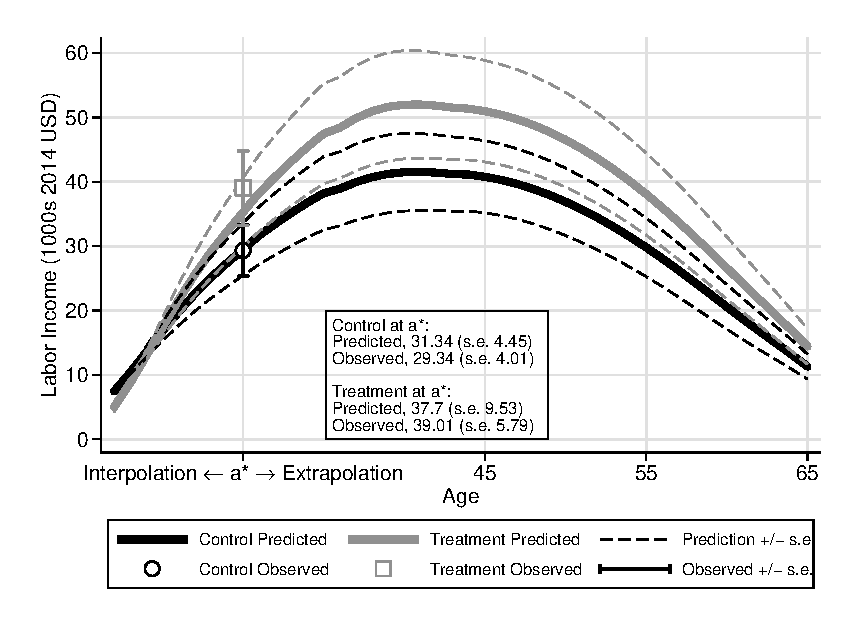
\includegraphics[width=\textwidth]{output/labor_25-65_pset1_mset1_male.eps}
\end{subfigure}%
\begin{subfigure}[h]{0.5\textwidth}
		\centering
		\caption{Females} \label{fig:labor-income-profilesa}
		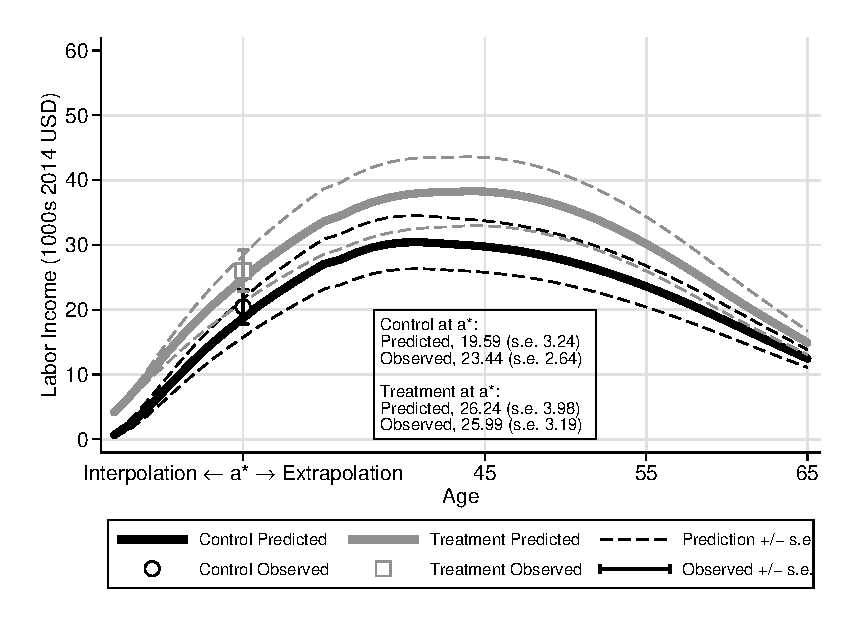
\includegraphics[width=\textwidth]{output/labor_25-65_pset1_mset1_female.eps}
\end{subfigure}
\footnotesize \justify
Note: Panel (a) displays the forecast life-cycle labor income profiles for ABC/CARE males by treatment status, based on the method proposed in Section~\ref{section:cbamethodology}. We combine data from the Panel Study of Income Dynamics (PSID), the National Longitudinal Survey of Youth 1979 (NLSY79), and the Children of the National Longitudinal Survey of Youth 1979 (CNLSY79). We highlight the \textit{observed} labor income at $a^*$ (age 30) for the ABC/CARE control- and treatment-group participants. Panel (b) displays the analogous figure for females. Our forecasts go up to age 67, the age of assumed retirement. Standard errors are the standard deviations of the empirical bootstrap distribution. See  Appendix~\ref{appendix:methodology} for a discussion of our choice of predictors and a sensitivity analysis on those predictors. We under-predict labor income for both males and females. These differences, however, are not statistically significant (and labor income is a relatively minor component of the overall analysis for females).
\end{sidewaysfigure}

\subsubsection{Alternative Forecasting Models for Labor Income} \label{section:sens}

\noindent An alternative non-parametric forecasting method compresses the whole forecasting procedure. Under Assumptions~\ref{ass:summary} and~\ref{ass:exog}, we can use matching on baseline variables and \emph{variables affected by treatment} to construct counterparts to the experimental treatment and control groups in the non-experimental sample.\footnote{\citet{Heckman_Ichimura_etal_1998_Econometrica} discuss this procedure.} Matching is a non-parametric estimation procedure for conditional mean functions. Matching creates direct counterparts in the auxiliary sample for \textit{each member} of the experimental sample. Instead of estimating a model for the life-cycle profile of labor income and forecasting from it, we directly use the counterpart matched profiles.\footnote{See Appendix~\ref{appendix:nonpar} for details.} This is an intuitively appealing non-parametric estimator of life-cycle program treatment effects that is valid under exogeneity \citep{Heckman_Navarro_2004_REStat}.

This is a fundamentally different matching procedure than what is used to construct the synthetic cohort in \textbf{Step 1}. In the main analysis of this paper, we match on baseline variables not affected by treatment to construct a synthetic cohort with $\bm{B} \in \mathcal{B}_0$. Using these samples, we estimate production functions on this cohort to forecast out-of-sample treatment effects. In contrast, in the analysis of this subsection, we match both on baseline variables and on variables affected by treatment compressing the construction of the synthetic cohort and the estimation of the production functions for out-of-sample forecasts to a single, non-parametric procedure.

Table~\ref{table:predsens} shows that there is close agreement between non-parametric estimates based on matching and the more parametric model-based approach previously presented. This reassuring concordance is consistent with exogeneity of inputs and structural invariance.

\section{Forecasting Other Life-cycle Benefits} \label{section:cbapractice}

\noindent In this section, we adapt the methodology described in Section~\ref{section:cbamethodology} to forecast the net benefits of the program arising from enhanced parental income, health, and reduced crime. In the text, we focus on forecasting health benefits and briefly discuss forecasts of crime and parental labor income.\footnote{Appendices~\ref{appendix:crime} and~\ref{app:parentalincome} provide further documentation.} Procedures for forecasting the benefits and costs of education are reported in Appendix~\ref{appendix:education}.

\subsection{Health}

\noindent One contribution of this paper is forecasting and monetizing the life-cycle benefits of the enhanced health and reduced health costs of participants using a version of Equation~\eqref{eq:outcome}. The model recognizes that: (i) health outcomes such as diabetes, heart disease, or death are absorbing states; and (ii) there is no obvious terminal time period for benefits and costs except death, which we forecast.

We adapt the Future Adult Model (FAM)---a forecasting model for health conditions and costs developed by Dana Goldman and coauthors \citep{Goldman_etal_2015_Future-Elderly-Model-Report}.\footnote{Appendix~\ref{appendix:health} discusses the FAM methodology in detail. It is not a competing risks model, but forecasts vectors of incidence and costs of disease one category at a time using univariate models.} We forecast health outcomes of program participants from their mid 30s up to their projected age of death.\footnote{The simulation starts at the age in which we observe the subjects' age-30 follow-up.} Our version of FAM passes a variety of specification tests and accurately forecasts health outcomes and health behaviors.\footnote{In Appendix~\ref{appendix:health-validation}, we present tests of the model assumptions and predictive performance for population aggregate health and health behavior outcomes.}

Our methodology has four steps--extensive details are provided in Appendix~\ref{appendix:health}: (i) follow an adapted version of the steps in Section~\ref{section:cbamethodology} to predict the state occupancy probabilities for the ABC/CARE subjects; (ii) estimate quality-adjusted life year (QALY) models using the Medical Expenditure Panel Survey (MEPS) and the PSID;\footnote{QALY is a measure which reweighs a year of life according to its quality given the burden of disease \citep{Dolan_1997_Modeling_MC,Shaw_etal_2005_EQ5D_MC}.} (iii) estimate medical cost models using MEPS and the Medicare Current Beneficiary Survey (MCBS), allowing estimates to differ by health state and observed characteristics; and (iv) forecast the medical expenditures and QALYs that correspond to the simulated individual health trajectories.\footnote{As part of step in (i), we impute some of the variables used to initialize the FAM models (see  Appendix~\ref{section:FAM_ABC_impute}).}

Our application of FAM uses the information on age-30 observed characteristics and a mid-30s health survey allowing us to account for components that are important for forecasting health outcomes. The models forecast the probability of having any of the major disease categories and health states at age $a+1$ based on the state of health as summarized by major disease categories at age $a$.\footnote{See Tables~\ref{table:supertab1} to~\ref{table:supertab3} for a summary. Our forecasts are based on two-year lags, due to data limitations in the auxiliary sources we use to simulate the FAM. For example, if the individual is 30 (31) years old in the age-30 interview, we simulate the trajectory of her health status at ages 30 (31), 32 (33), 34 (35), and so on until her projected death. Absorbing states are an exception. For example, heart disease at age $a$ does not enter in the estimation of transitions for heart disease at age $a+1$ because it is an absorbing state: once a person has heart disease, she carries it through the rest of her life.}

Using the occupancy probabilities for each health outcome at each age, we take a Monte-Carlo draw for each subject. Each simulation depends on each individual's health history and on her characteristics. For every simulated trajectory of health outcomes, we forecast the life-cycle medical expenditure using the models estimated from the MEPS and the MCBS. We estimate the expected life-cycle medical expenditure by taking the mean of each individual's simulated life-cycle medical expenditure.

The models estimated using MCBS represent medical costs in the years 2007 to 2010. The MEPS estimation captures costs during 2008 to 2010. To account for real medical cost growth after 2010, we adjust each model's forecast using the method described in  Appendix~\ref{appendix:health-fam-simulation}. The same procedure is applied to calculate QALYs. We compare QALY based on a widely-used health-related Quality-of-Life measure available in MEPS.\footnote{HRQoL measure EQ-5D.} We then apply this model to the PSID data. QALYs monetize the health of an individual at each age. Although there is not a clear age-by-age treatment effect on QALYs, there is a statistically and substantively significant difference in the accumulated present value of the QALYs between the treatment and the control groups.\footnote{Our baseline estimation assumes that each year of life is worth  $\$150,000$ (2014 USD). Our estimates are robust to substantial variation in this assumption, as we show in  Appendix~\ref{appendix:sensitivity}.}

We estimate three models of medical spending: (i) Medicare spending (annual medical spending paid by parts A, B, and D of Medicare); (ii) private spending (medical spending paid by a private insurer or paid out-of-pocket by the individual); and (iii) all public spending other than Medicare. Each medical spending model includes the variables we use to forecast labor and transfer income, together with current health, risk factors, and functional status as explanatory variables.

We also calculate medical expenditures before age 30.\footnote{See Appendix~\ref{appendix:health-costs-before-age30}.} The ABC/CARE interviews at ages 12, 15, 21 and 30 have information related to hospitalizations at different ages and number of births before age 30. We combine this information along with individual and family demographic variables to use MEPS to forecast medical spending for each age.

\subsection{Crime}

\noindent To estimate the life-cycle benefits and costs of ABC/CARE on crime, we use rich data obtained from public records. Two previous studies consider the impacts of ABC on crime: \citet{Clarke_Campbell_1998_ABC_Comparison_ECRQ} use administrative crime records up to age 21, and find no statistically significant treatment effects. \cite{Barnett_Masse_2002_benefitcost,Barnett_Masse_2007_EER} analyze self-reported crime at age 21. They lacked access to the longer-term, administrative data that we use and report weak treatment effects on crime. Our study improves on this research in two ways: (i) we use administrative data on the accumulated number of crimes that participants commit through their mid 30s; (ii) we use micro-data specific to the states in which participants grew up, as well as other national datasets, to forecast criminal activity from the mid 30s to 50. We forecast using methods standard in the criminology literature.\footnote{\citet{Cohen-Bowles_2010_Estimating-Cost-Crime} and \citet{McCollister_etal_2010_DAD}.} See Appendix~\ref{appendix:crime} for a a complete discussion of our crime forecasts.

\subsection{Parental Labor Income} \label{section:pincome}

\noindent ABC/CARE offers childcare to the parents of treated children for more than nine hours a day for five years, 50 weeks a year. Only $27\%$ of participant mothers of children reported living with a partner at baseline. This barely changed during the course of the experiment (see Appendix~\ref{appendix:background}). The childcare component generates substantial treatment effects on maternal labor force participation and parental labor income.\footnote{There is also an effect on maternal school enrollment. Some of the mothers decided to enroll in school and further their education. This could be one of the reasons why they make more money afterward. We report these treatment effects in Appendix~\ref{appendix:background}. We quantify the social cost of additional education in Appendix~\ref{appendix:education}.} In addition, subsidized childcare induced wage growth due to enhanced parental educational attainment and through wage growth due to work experience.

We observe parental labor income at eight different ages for the participants through age 21.\footnote{The ages at which parental labor income is observed are 0, 1.5, 3.5, 4.5, 8, 12, 15, and 21. At age 21 the mothers of the ABC/CARE subjects were, on average, 41 years old.}$^,$\footnote{We linearly interpolate parental labor income for ages for which we do not have observations between 0 and 21.} To estimate the profile of parental earnings over the entire life-cycle, we use two different approaches in Appendix~\ref{app:parentalincome}: (i) an approach based on projections using standard Mincer equations; and (ii) an approach based on the analysis of Section~\ref{section:cbamethodology}.

Any childcare inducements of the program likely benefit parents who, at baseline, did not have any other children who were not eligible for program participation. Additional childcare responsibilities would weaken the childcare effects of ABC/CARE, especially if younger siblings are present. In Appendix~\ref{app:parentalincome}, we show that the treatment effect for discounted parental labor income is much larger when participant children have no siblings at baseline. Treatment effects weaken when comparing children who have siblings younger than 5 years old to children who have siblings age 5 years or older.\footnote{These patterns persist when splitting the ABC/CARE sample by gender, but the estimates are not precise because the samples become too small. See Appendix~\ref{app:parentalincome}.}

\subsection{Program Costs} \label{section:programscosts}

\noindent The yearly cost of the program was \$18,514 per participant in 2014 USD. We improve on previous cost estimates by using primary-source documents.\footnote{Our calculations are based on progress reports written by the principal investigators and related documentation recovered in the archives of the research center where the program was implemented. We display these sources in Appendix~\ref{app:programcosts}. The main component is staff costs. Other costs arise from nutrition and services that the subjects receive when they were sick, diapers during the first 15 months of their lives, and transportation to the center. The control-group children also receive diapers during approximately 15 months, and iron-fortified formula. The costs are based on sources describing ABC treatment for $52$ children. We use the same costs estimates for CARE, for which there is less information available. The costs exclude any expenses related to research or policy analysis. A separate calculation by the implementers of the program indicates almost an identical amount (see  Appendix~\ref{app:programcosts}).} Appendix~\ref{app:programcosts} discusses program costs in detail.

\section{Estimates and Sensitivity Analysis} \label{section:cbaresults}

\noindent Figure~\ref{figure:main} summarizes our findings. It displays the discounted (using a 3\% discount rate) life-cycle benefits and costs of the program (2014 USD) pooled across genders, over all outcome categories, and for separate categories as well.\footnote{Using discount rates of 0\%, 3\%, and 7\%, the estimates for the benefit/cost ratios are 17.40 (s.e.\ 5.90), 7.33 (s.e.\ 1.84), and 2.91 (s.e.\ 0.59), respectively. We report estimates for discount rates between 0\% and 15\% in  Appendix~\ref{appendix:varying-discount-rate}.} These benefits are the inputs of our baseline estimates for the annual internal rates of return and benefit/cost ratios. We conduct extensive sensitivity and robustness analyses to produce ranges of plausible values for the estimates of the internal rate of return (8.0,\ 18.3) and benefit/cost ratio (1.52,\ 17.40).

The costs of the program are substantial, as frequently been noted by critics.\footnote{See, e.g., \citet{Fox_News_2014_Head_Start_Effects} and \citet{Whitehurst_2014_Senate_Testimony}.} But so are the benefits, which far outweigh the costs. The individual gains in labor income, parental labor income, crime, and health are at least as large in magnitude as the costs. As a consequence, our measures of social efficiency remain statistically and economically significant even after eliminating the benefits from any one of the four main components that we monetize. No single component drives our results.

\begin{sidewaysfigure}[!htbp]
\caption{Net Present Value of Main Components of the Pooled (Over Gender) Cost/Benefit Analysis Over the Life Cycle per Program Participant, Treatment vs. Control}\label{figure:main}
\centering
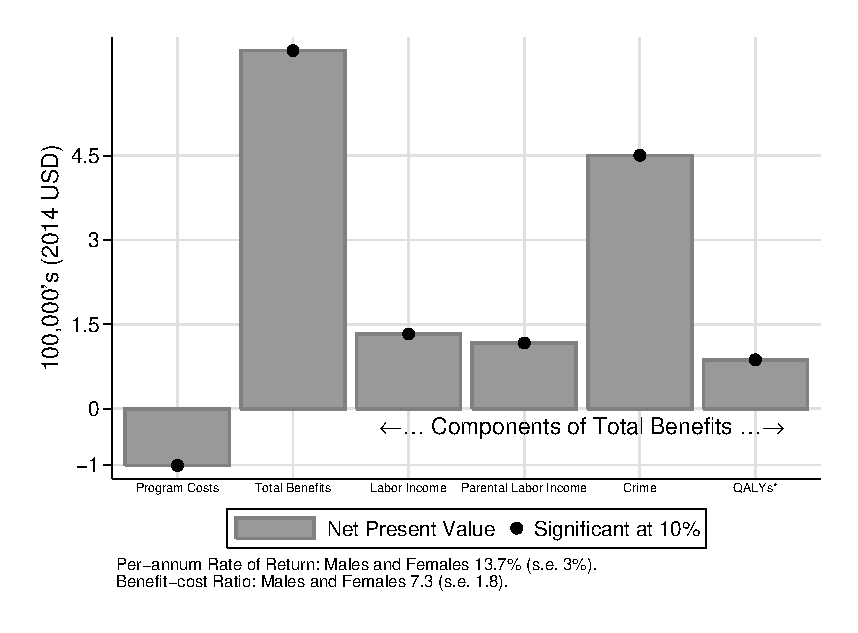
\includegraphics[width=.7\columnwidth]{output/abccare_npvssummredux.eps}
\footnotesize \justify
Note: This figure displays the life-cycle net present values per program participant of the main components of the cost/benefit analysis of ABC/CARE from birth to forecasted death, discounted to birth at a rate of 3\%. By ``net" we mean that each component represents the total value for the treatment group minus the total value for the control group. Program costs: the total cost of ABC/CARE, including the welfare cost of taxes to finance it. Total benefits: the benefits for \textit{all} of the components we consider. Labor income: total individual labor income from age 21 to the retirement of program participants (assumed to be at age 67). Parental labor income: total parental labor income of the parents of the participants from when the participants were ages 1.5 to 21. Crime: the total cost of crime (judicial and victimization costs). To simplify the display, the following components are not shown in the figure: (i) cost of alternative preschool paid by the control-group children's parents; (ii) the social welfare costs of transfer income from the government; (iii) disability benefits and social security claims; (iv) costs of increased individual and maternal education (including special education and grade retention); (v) total medical public and private costs. Inference is based on non-parametric, one-sided $p$-values from the empirical bootstrap distribution. Dots $(\bullet)$ indicate point estimates significant at the $10\%$ level.
*QALYs refers to the quality-adjusted life years. Any gain corresponds to better health conditions until forecasted death, with $\$150,000$ (2014 USD) as the base value for a year of life.
\end{sidewaysfigure}

Pooling males and females, the program is socially efficient: the internal rate of return and the benefit/cost ratio are $13.7\%$ and $7.3$, respectively. These estimates are statistically significant, even after accounting for sampling variation and forecast and estimation error in the experimental and auxiliary samples and the tax costs of financing the program.\footnote{We obtain the reported standard errors by bootstrapping \emph{all} steps of our empirical procedure, including variable selection, imputation, model selection steps, and forecast error (see  Appendix~\ref{appendix:bootstrap}).}

We conduct an extensive set of sensitivity analysis. Table~\ref{table:bcsens} displays the results of a sensitivity analysis of the estimates of the benefit/cost ratio to alternative plausible assumptions. Table~\ref{table:irrsens} presents the corresponding internal rates of return. Our estimates are not driven by our methods for accounting for attrition and item non-response, by the conditioning variables, by the functional forms of projection equations used when computing the net-present values or by values of externally set parameters, such as the value of life introduced in our predictions of crime and health costs.\footnote{See Appendix~\ref{appendix:methodology} for a detailed discussion.} Although the internal rate of return remains relatively high when using participant outcome measures only up to ages 21 or 30, the benefit/cost ratios indicate that accounting for benefits that go beyond age 30 is important. The return to each dollar is at most $3/1$ when only considering benefits up to age 30 (see the columns in the forecast span rows).

Accounting for the treatment substitutes available to controls also matters. Males benefit the most from ABC/CARE relative to attending alternative formal childcare, while females benefit the most from ABC/CARE relative to staying at home. We explore these differences futher in Appendix~\ref{appendix:cbaresultscont}.

\begin{sidewaystable}[!htpb]
\begin{threeparttable}
\caption{Sensitivity Analysis for Benefit/Cost Ratios}
\label{table:bcsens}
\centering
\scriptsize
\begin{tabularx}{22.5cm}{XcX}
& \begin{tabular}{>{\bfseries}lcc|cc|cc} \toprule
	&	\multicolumn{2}{c}{\textbf{\textit{Pooled}}}	&	\multicolumn{2}{c}{\textbf{\textit{Males}}}	&	\multicolumn{2}{c}{\textbf{\textit{Females}}}	\\ 
Baseline	&	\multicolumn{2}{c}{5.69 (s.e. 2.32)}	&	\multicolumn{2}{c}{11.62 (s.e. 5.49)}	&	\multicolumn{2}{c}{2.60 (s.e. 0.98)}	\\ \\
\multicolumn{7}{l}{\textit{Baseline: IPW and Controls, Life-span up to Age 79, Treatment vs. Next Best, 50\% Marginal tax 50\% (deadweight loss), Discount rate 3\%, Parental}} \\	
\multicolumn{7}{l}{\textit{income 0 to 21 (child's age), Labor Income predicted from 21 to 65, All crimes (full costs), Value of life 150,000.}} \\ \\ \midrule	
Specification	&	\textit{No IPW}	&	\textit{and No Controls}	&	\textit{No IPW}	&	\textit{and No Controls}	&	\textit{No IPW}	&	\textit{and No Controls}	\\
	&	\textbf{6.17}	&	\textbf{5.35}	&	\textbf{11.94} 	&	\textbf{10.74}	&	\textbf{2.91}	&	\textbf{2.79}	\\
	&	(2.35)	&	(2.04)	&	(6.14)	&	(4.12)	&	(0.97)	&	(0.81)	\\ \midrule
Prediction	&	\textit{to Age 21}	&	\textit{to Age 30}	&	\textit{to Age 21}	&	\textit{to Age 30}	&	\textit{to Age 21}	&	\textit{to Age 30}	\\
Span	&	\textbf{1.55}	&	2.01	&	\textbf{2.17}	&	2.80	&	1.17	&	1.52	\\
	&	(0.39)	&	(0.88)	&	(0.74)	&	(1.96)	&	(0.43)	&	(0.48)	\\ \midrule
Counter-	&	\textit{vs. Stay at Home}	&	\textit{vs. Alt. Presch.}	&	\textit{vs. Stay at Home}	&	\textit{vs. Alt. Presch.}	&	\textit{vs. Stay at Home}	&	\textit{vs. Alt. Presch.}	\\
factuals	&	\textbf{4.44}	&	\textbf{6.58}	&	3.88	&	\textbf{10.85}	&	\textbf{4.89}	&	\textbf{2.40}	\\
	&	(1.68)	&	(2.22)	&	(2.78)	&	(4.14)	&	(1.50)	&	(0.94)	\\ \midrule
Deadweight-	&	\textit{0\%}	&	\textit{100\%\textit}	&	\textit{0\%}	&	\textit{100\%\textit}	&	\textit{0\%}	&	\textit{100\%\textit}	\\
loss	&	\textbf{8.50}	&	\textbf{4.29}	&	\textbf{17.43}	&	\textbf{8.71}	&	\textbf{3.69}	&	2.06	\\
	&	(3.47)	&	(1.75)	&	(8.19)	&	(4.14)	&	(1.43)	&	(0.79)	\\ \midrule
Discount 	&	\textit{0\%}	&	\textit{7\%}	&	\textit{0\%}	&	\textit{7\%}	&	\textit{0\%}	&	\textit{7\%}	\\
Rate	&	13.38	&	2.40	&	29.50	&	4.21	&	5.34	&	1.43	\\
	&	7.01	&	0.80	&	15.93	&	1.88	&	3.81	&	0.37	\\ \midrule
Parental	&	\textit{Mincer Life-cycle}	&	\textit{Life-cycle Prediction}	&	\textit{Mincer Life-cycle}	&	\textit{Life-cycle Prediction}	&	\textit{Mincer Life-cycle}	&	\textit{Life-cycle Prediction}	\\
Income	&	\textbf{5.92}	&	\textbf{5.60}	&	\textbf{11.80}	&	\textbf{12.36}	&	\textbf{2.88}	&	\textbf{3.27}	\\
	&	(2.32)	&	(2.39)	&	(5.49)	&	(5.68)	&	(1.02)	&	(1.21)	\\ \midrule
Labor	&	\textit{.5\% Annual Decay}	&	\textit{.5\% Annual Growth}	&	\textit{.5\% Annual Decay}	&	\textit{.5\% Annual Growth}	&	\textit{.5\% Annual Decay}	&	\textit{.5\% Annual Growth}	\\
Income	&	\textbf{5.48}	&	\textbf{5.90}	&	\textbf{10.76}	&	\textbf{12.49}	&	\textbf{2.47}	&	\textbf{2.74}	\\
	&	(2.25)	&	(2.41)	&	(5.33)	&	(5.71)	&	(0.87)	&	(1.10)	\\ \midrule
Crime	&	\textit{Drop Major Crimes}	&	\textit{Halve Costs}	&	\textit{Drop Major Crimes}	&	\textit{Halve Costs}	&	\textit{Drop Major Crimes}	&	\textit{Halve Costs}	\\
	&	\textbf{5.14} 	&	\textbf{4.07}	&	\textbf{11.82}	&	\textbf{8.33}	&	\textbf{2.72}	&	2.25	\\
	&	(2.30)	&	(1.50)	&	(5.59)	&	(3.64)	&	(1.04)	&	(0.95)	\\ \midrule
Health	&	\textit{Drop All}	&	\textit{Double Value of Life}	&	\textit{Drop All}	&	\textit{Double Value of Life}	&	\textit{Drop All}	&	\textit{Double Value of Life}	\\
(QALYs)	&	\textbf{4.85}	&	\textbf{6.56}	&	\textbf{10.61}	&	\textbf{12.63}	&	\textbf{2.48}	&	2.73	\\
	&	(2.32)	&	(2.54)	&	(5.37)	&	(5.90)	&	(0.97)	&	(1.26)	\\ \bottomrule
\end{tabular}  & \end{tabularx}
\begin{tablenotes}
\scriptsize
\item Note: This table displays sensitivity analyses of our baseline benefit/cost ratio calculation to the perturbations indexed in the different rows. The characteristics of the \textit{baseline} calculation are in the table header. IPW: adjusts for attrition and item non-response (see  Appendix~\ref{app:method_partialobs} for details). Control variables: Apgar scores at ages 1 and 5 and a high-risk index (see  Appendix~\ref{appendix:results} for details on how we choose these controls). When forecasting up to ages 21 and 30, we consider all benefits and costs up to these ages, respectively. Counterfactuals: we consider treatment vs. next best (baseline), treatment vs. stay at home, and treatment vs. alternative preschools (see Appendix~\ref{appendix:cbaresultscont} for a discussion). Deadweight loss is the loss implied by any public expenditure (0\% is no loss and 100\% is one dollar loss per dollar spent). Discount rate: rate to discount benefits to child's age 0 (in all calculations). Parental labor income: see  Appendix~\ref{app:parentalincome} for details on the two alternative forecasts (Mincer and Life-cycle). Labor Income: 0.5\ annual growth (decay) is an annual wage growth (decay) due to cohort effects. Crime: major crimes are rape and murder; half costs takes half of victimization and judiciary costs. Health (QALYs): ``drop all'' sets the value of life equal to zero. Standard errors obtained from the empirical bootstrap distribution are in parentheses. Bolded $p$-values are significant at 10\% using one-sided tests. For details on the null hypothesis see Table~\ref{table:cba}.
\end{tablenotes}
\end{threeparttable}
\end{sidewaystable}

\begin{sidewaystable}[!htpb]
\begin{threeparttable}
\caption{Sensitivity Analysis for Internal Rate of Return}
\label{table:irrsens}
\centering
\scriptsize
\begin{tabularx}{22.5cm}{XcX}
& % matrix: allirr file: allirr_sens.tex  25 Sep 2016 09:11:16
\begin{table}[htbp]
\begin{tabular}{lcccccc} \hline \hline
 & pooled  & pooled  & males  & males  & females  & females  \\  \hline 
baseline &     0.087 &     0.052 &     0.138 &     0.048 &     0.126 &     0.048 \\  
specification &     0.092 &     0.087 &     0.147 &     0.148 &     0.136 &     0.122 \\  
. &     0.059 &     0.032 &     0.060 &     0.037 &     0.044 &     0.039 \\  
predictiontime &     0.099 &     0.127 &     0.110 &     0.127 &     0.104 &     0.115 \\  
. &     0.056 &     0.051 &     0.047 &     0.051 &     0.045 &     0.043 \\  
counterfactual &     0.131 &     0.089 &     0.085 &     0.162 &     0.100 &     0.132 \\  
. &     0.046 &     0.057 &     0.038 &     0.044 &     0.034 &     0.039 \\  
dwl &     0.128 &     0.068 &     0.175 &     0.118 &     0.174 &     0.103 \\  
. &     0.089 &     0.037 &     0.063 &     0.042 &     0.064 &     0.037 \\  
parental &     0.104 &         . &     0.148 &         . &     0.142 &         . \\  
. &     0.069 &         . &     0.053 &         . &     0.053 &         . \\  
lincome &     0.080 &         . &     0.127 &         . &     0.122 &         . \\  
. &     0.053 &         . &     0.054 &         . &     0.047 &         . \\  
crime &     0.089 &     0.081 &     0.153 &     0.122 &     0.124 &     0.110 \\  
. &     0.052 &     0.051 &     0.043 &     0.046 &     0.044 &     0.044 \\  
health &     0.091 &     0.085 &     0.136 &     0.134 &     0.112 &     0.127 \\  
. &     0.053 &     0.052 &     0.049 &     0.053 &     0.058 &     0.045 \\  
\hline \hline \end{tabular}
\end{table}
 & \end{tabularx}
\begin{tablenotes}
\footnotesize
\item Note: This table displays sensitivity analyses of our baseline internal rate of return calculation to the perturbations indexed in the different rows. The characteristics of the \textit{baseline} calculation are in the table header. IPW: adjusts for attrition and item non-response (see  Appendix~\ref{app:method_partialobs} for details). Control variables: Apgar scores at ages 1 and 5 and a high-risk index (see  Appendix~\ref{appendix:results} for details on how we choose these controls). When forecasting up to ages 21 and 30, we consider all benefits and costs up to these ages, respectively. Counterfactuals: we consider treatment vs. next best (baseline), treatment vs. stay at home, and treatment vs. alternative preschools (see Appendix~\ref{appendix:cbaresultscont} for a discussion). Deadweight loss is the loss implied by any public expenditure (0\% is no loss and 100\% is one dollar loss per dollar spent). Parental labor income: see  Appendix~\ref{app:parentalincome} for details on the two alternative forecasts (Mincer and Life-cycle). Labor Income: 0.5\ annual growth is an annual wage growth due to cohort effects; only benefit assumes labor income is the only benefit of the program. Crime: major crimes are rape and murder; half costs takes half of victimization and judiciary costs. Health (QALYs): ``drop all'' sets the value of life equal to zero. Bolded $p$-values are significant at 10\% using one-sided tests. For details on the null hypothesis see Table~\ref{table:cba}.
\end{tablenotes}
\end{threeparttable}
\end{sidewaystable}

Our baseline estimates account for the deadweight loss caused by distortionary taxes collected to fund programs, plus the direct costs associated with collecting taxes.\footnote{When the transaction between the government and an individual is a direct transfer, we consider 0.5 as the cost per each transacted dollar. We do not weight the final recipient of the transaction (e.g., transfer income). When the transaction is indirect, we classify it as government spending as a whole and consider its cost as 1.5 per dollar spent (e.g., public education).} We assume a marginal tax rate of $50\%$.\footnote{\citet{Feldstein_1999_REStat} estimates that the deadweight loss caused by increasing existing tax rates (marginal deadweight loss) may exceed two dollars per dollar of revenue generated. We use a more conservative value (0.5 dollars per dollar of revenue generated). In Tables~\ref{table:bcsens}, \ref{table:irrsens}, and in  Appendix~\ref{appendix:varying-dwl}, we explore the robustness of this choice of the welfare cost and find little sensitivity.} Our estimates are robust to dropping it to $0\%$ or doubling it to $100\%$ (deadweight loss columns). Our baseline estimate of benefit/cost ratios is based on a discount rate of $3\%$. Not discounting roughly doubles our benefit/cost ratios, while they remain statistically significant using a higher discount rate of $7\%$ (discount rate columns).

Parental labor income effects induced by the childcare subsidy are an important component of the benefit/cost ratio. We take a conservative approach in our baseline estimates and do not account for potential shifts in parental labor income profiles due to education and work experience subsidized by childcare (see the discussion in Section~\ref{section:pincome}). Our baseline estimates rely solely on parental labor income when participant children are ages 0 to 21. Alternative approaches considering the gain for the parents through age 67 generate an additional increase in the gain due to parental labor income (see parental labor income columns).\footnote{If labor markets operate without frictions and the marginal rate of substitution between leisure and consumption equals the marginal wage rate, parental labor income should not be valued at the margin. The bottom box of Figure~\ref{figure:vennpooled} shows that the benefit/cost ratio and the internal rate of return remain sizable in magnitude and statistically significant if we omit parental income from the benefits attributed to the program.}

Individuals in ABC/CARE could experience positive cohort effects that might (i) make them more productive and therefore experience wage growth; (ii) experience a negative shock such as an economic crisis and therefore experience a wage decline. Our estimates are robust when we vary annual growth and decay rates in labor income between $-0.5\%$ and $0.5\%$. This is consistent with the range of values in \citet{Lagakos_Moll_etal_2016_LifeCycle_NBER}.

We also examine the sensitivity of our estimates to (i) dropping the most costly crimes such as murders and rapes;\footnote{Two individuals in the treatment group were convicted of rape and one individual in the control group was convicted of murder.} and (ii) halving the costs of victimization and judiciary costs related to crime. The first sensitivity check is important because we do not want our estimates to be based on a few exceptional crimes. The second is important because estimates of victimization costs are controversial because they are subjective (see  Appendix~\ref{appendix:crime-VI}). Our benefit/cost estimates are robust to these adjustments, even though crime is a major component of it. We also examine the sensitivity with respect to our main health component: quality-adjusted life years. This is an important component because healthier individuals survive longer, and treatment improves health conditions. Since this component is largely realized later in life and thus is heavily discounted, improvements in future medical care have a negligible effect on the estimated life-cycle benefits. Dropping this component or doubling the value of life does not have a major impact on our calculations.

Figure~\ref{figure:vennpooled} summarizes the results from our extensive sensitivity analyses reported in Table~\ref{table:cba} of Appendix~\ref{appendix:sensitivity}, including the case where only one of the many streams we consider is the source of the benefit. We calculate the estimates with all possible combinations of the main benefit and cost streams. Our measures of economic efficiency remain statistically and economically significant even after eliminating the benefits from any one of the four main components that we monetize.  Overall, our sensitivity analyses indicate that no single category of outcomes drives the social efficiency of the program. Rather, it is the life-cycle benefits across multiple dimensions of human development.

\begin{figure}[htpb!]
\caption{Benefit/Cost Ratio and Internal Rate of Return when Accounting for Different Combinations of the Main Benefits}\label{figure:vennpooled}
\centering
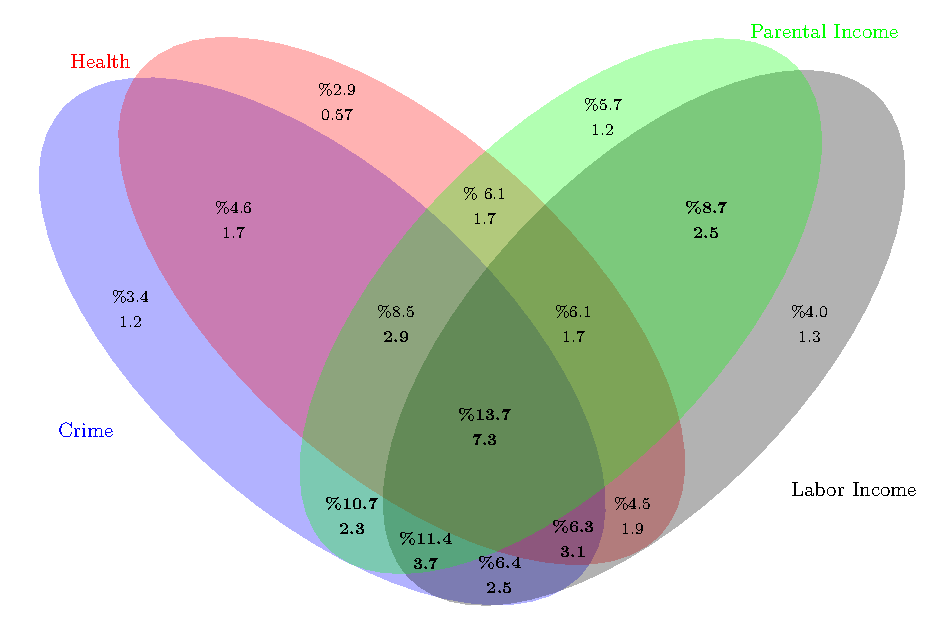
\includegraphics[width=.7\columnwidth]{output/venn_pooled.pdf}
\footnotesize \justify
Note: This figure presents all possible combinations of accounting for the benefits from the four major categories in our analysis. The non-overlapping areas present estimates arising from a single category as the benefit. Where multiple categories overlap, we account for benefits from each of the overlapping categories. The other components remain constant across all calculations and are the same as in Figure~\ref{figure:main}. Health combines QALYs (quality-adjusted life years) and health expenditure. Inference is based on non-parametric, one-sided $p$-values from the empirical bootstrap distribution. We put boxes around point estimates that are statistically significant at the $10\%$ level.
\end{figure}

\section{Assessing Recent Benefit-Cost Analyses} \label{section:bcaestimates}

\noindent We use our analysis to examine the empirical foundations of the approach to benefit/cost analysis taken in a prototypical study of \citet{Kline_Walters_2016_QJE}, which in turn is based on estimates taken from \citet{Chetty_Friedman_etal_2011_QJoE}.\footnote{Examples of application of this approach include \citet{Attanasio_Kugler_Meghir_2011_AEJAE}, \cite{Behrman-et-al_2011_JHR-Progresa}, and \cite{Lafortune_etal_2018_Reform_AEJAE}.} Although widely emulated, this approach offers an imprecise approximation of benefit/cost ratios with questionable validity.

\citet{Kline_Walters_2016_QJE} use data from the Head Start Impact Study (HSIS) and report a benefit/cost ratio between $1.50$ and $1.84$.\footnote{HSIS is a one-year-long randomized evaluation of Head Start \citep{Puma_Bell_etal_2010_HeadStartImpact}.} Their analysis proceeds in three steps: (i) calculate program treatment effects on cognitive test scores measured around age 5;\footnote{They use an index based on the Peabody Picture Vocabulary and Woodcock Johnson III Tests.} (ii) monetize this gain using the return to cognitive test scores measured between ages 5 and 7 in terms of net present value of labor income at age 27 using the estimates of \citet{Chetty_Friedman_etal_2011_QJoE};\footnote{The \citet{Chetty_Friedman_etal_2011_QJoE} return is based on Stanford Achievement Tests.}$^,$\footnote{For this comparison exercise, we interpret the earnings estimated in \citet{Chetty_Friedman_etal_2011_QJoE} to be equivalent to labor income.}$^,$\footnote{Calculations from \citet{Chetty_Friedman_etal_2011_QJoE} indicate that a 1 standard deviation gain in achievement scores at age 5 implies a $13.1\%$ increase in the net present value of labor income through age 27. This is based on combining information from Project Star and administrative data at age 27.} and (iii) calculate the benefit/cost ratio based on this gain and their own calculations of the program's cost.\footnote{Their calculation assigns the net present value of labor income through age 27 of $\$385,907.17$ to the control-group participants, as estimated by  \citet{Chetty_Friedman_etal_2011_QJoE}.}$^,$\footnote{All monetary values that we provide in this section are in 2014 USD. We discount the value provided by \citet{Chetty_Friedman_etal_2011_QJoE} to the age of birth of the children in our sample (first cohort).}

\begin{table}[!htpb]
\begin{threeparttable}
\caption{Examining the Validity of Recent \emph{Ad Hoc} Methods for Forecasting in Light of the Analysis of This Paper}
\label{table:comparing}
\centering
\footnotesize
\begin{tabularx}{16.5cm}{XcX}
& \begin{tabular}{ccccc}
\toprule
(1) & (2) & (3) & (4) & (5)\\ \midrule
Age & \mc{1}{c}{NPV Source} & Component & \citet{Kline_Walters_2016_QJE} & Authors' Method \\
& & & Method & \\ \midrule
\multirow{2}{*}{27} & \cite{Chetty_Friedman_etal_2011_QJoE} & Labor income & 0.58 (s.e. 0.28) &  \\
& ABC/CARE-calculated & Labor income & 0.09 (s.e. 0.04) &  1.09 (s.e. 0.04)\\ \\
\multirow{2}{*}{34} & ABC/CARE-calculated & Labor income & 0.37 (s.e. 0.04) & 0.15 (s.e. 0.05) \\
& ABC/CARE-calculated & All & 1.21 (s.e. 0.05) &  3.20 (s.e. 1.04) \\ \\
\multirow{2}{*}{Life-cycle} &  ABC/CARE-calculated & Labor income & 1.56 (s.e. 0.08) & 1.55 (s.e. 0.76) \\
& ABC/CARE-calculated & All & 3.80 (s.e. 0.29) & 7.33 (s.e. 1.84) \\
\bottomrule
\end{tabular}
&
\end{tabularx}
\begin{tablenotes}
\footnotesize
\item Note: This table displays benefit/cost ratios based on the methodology in \citet{Kline_Walters_2016_QJE} and based on our own methodology. Age: age at which we stop calculating the net present value. NPV Source: source where we obtain the net present value. Component: item used to compute net present value (all refers to the net present value of all the components). \citet{Kline_Walters_2016_QJE} Method: estimate based on these authors' methodology. Authors' Method: estimates based on our methodology. Standard errors are based on the empirical bootstrap distribution.
\end{tablenotes}
\end{threeparttable}
\end{table}

To analyze how our estimates compare to those based on this method, we present a series of estimates in the fourth column of Table~\ref{table:comparing}. For purposes of comparison, the fifth column of Table~\ref{table:comparing} shows the analogous estimates based on our samples and forecasts.

For the first estimate, we calculate the benefit/cost ratio using both the ``return to IQ'' and the net present value of labor income at age 27 reported in \citet{Chetty_Friedman_etal_2011_QJoE}. This calculation is the same type of calculation as that used in \citet{Kline_Walters_2016_QJE}. In the second exercise, we perform a similar exercise but use our own estimate of the net present value of labor income at age 27.\footnote{This allows us to compute our own ``return to IQ'' and impute it to the treatment-group individuals.} In this exercise, the standard errors account for variation in the return because we calculate the return in every bootstrapped re-sample. In that sense, our approach more accurately accounts for the underlying uncertainties when compared to the approach of \citet{Kline_Walters_2016_QJE}, who do not account for estimation error in reporting standard errors. The estimated return is smaller because our sample is much more disadvantaged than that used by \citet{Chetty_Friedman_etal_2011_QJoE}.

The remaining exercises in Table~\ref{table:comparing} are: (i) increase the age range over which we calculate the net-present value of labor income; or (ii) consider the value of all the components we analyze throughout the paper, in addition to labor income. The more inclusive the benefits measured and the longer the horizon over which they are measured, the greater the benefit/cost ratio. The final reported estimate, 7.3, is our baseline estimate that incorporates all of the components across the life cycles of the subjects.

Our methodology provides a more accurate estimate of the benefits and costs of the ABC/CARE program. We better quantify the effects of the experiment by considering the multiplicity of benefits over the whole life cycle. We also better approximate the uncertainty of our estimates by considering both the sampling error in the experimental and auxiliary samples, the forecast error due to the interpolation and extrapolation, and the sensitivity of the estimates to externally specified parameters.

\section{Summary} \label{section:conclusion}

\noindent This paper presents a template for constructing economically interpretable summaries of the multiple treatment effects generated from a randomized evaluation of a high-quality, widely emulated early childhood program with follow-up through the mid 30s. We go beyond the usual practice of reporting batteries of treatment effects. We report the costs and monetize the treatments across numerous domains. We estimate the tax-adjusted internal rate of return and the benefit/cost ratio of the program. These aggregates assess the social efficiency of the program.

We use auxiliary information and economic models to guide monetization of treatment effects and to extrapolate the measured benefits and costs to the full life cycles of participants. We account for model estimation and forecast error and conduct extensive sensitivity analyses of our estimates to alternative assumptions and methodologies. Under a variety of plausible assumptions, we estimate that the tax-adjusted internal rate of return of the program ranges from 1.5\% to 17.4\%. These estimates demonstrate the social profitability of ABC/CARE.

We conclude with a cautionary note. The program we study was targeted to a disadvantaged, predominately African-American population in a university town in North Carolina. Blind generalization of our findings to other populations is clearly not warranted. In particular, there is no support in this study for universal application of ABC/CARE across all socio-economic groups.

However, the essential features of the ABC/CARE approach are currently in wide use in a variety of early childhood intervention programs that target disadvantaged children. In this sense, our analysis has lessons of general applicability to disadvantaged populations. Our study indicates what is possible and that the possibilities are substantial.

%References
\singlespace
\bibliographystyle{chicago}
\bibliography{heckman}

\end{document}

